\documentclass{beamer}

\usetheme{Madrid} % Singapore, Madrid, Ilmenau, CambridgeUS
\setbeamertemplate{navigation symbols}{}

% --- Colores personalizados ---
\definecolor{unahurverde}{HTML}{005C5C}
\definecolor{unahurgris}{HTML}{EAEAEA}
\setbeamercolor{structure}{fg=unahurverde}
\setbeamercolor{frametitle}{bg=unahurverde, fg=white}
\setbeamercolor{title}{fg=unahurverde}
\setbeamercolor{block title}{bg=unahurverde, fg=white}
\setbeamercolor{block body}{bg=unahurgris, fg=black}

% --- Logo en esquina superior derecha ---
\addtobeamertemplate{frametitle}{}{%
	\begin{textblock*}{3cm}(11.88cm,0.12cm)
		
\includegraphics[height=0.7cm]{logo_unahur.png}
	\end{textblock*}
}

\setbeamertemplate{caption}[numbered]


\usepackage[utf8]{inputenc}
\usepackage[spanish]{babel}
\usepackage{graphicx}
\usepackage{ragged2e}
\usepackage[table]{xcolor}
\usepackage{listings}
\usepackage{caption}
%\usepackage{enumitem}
\usepackage[absolute,overlay]{textpos} % Necesario para el logo

\usefonttheme[onlymath]{serif}

\definecolor{codegray}{rgb}{0.5,0.5,0.5}
\definecolor{backcolor}{rgb}{0.95,0.95,0.95}
\definecolor{verdecelda}{HTML}{B7CBA6}
\definecolor{rojocelda}{HTML}{FF9999}
\definecolor{lightgray}{gray}{0.6}

\definecolor{codebg}{rgb}{0.95,0.97,0.98}       % fondo celeste muy suave
\definecolor{codecomment}{rgb}{0.42,0.55,0.34}  % verde oliva suave y cursiva
\definecolor{codekeyword}{rgb}{0.0,0.45,0.73}    % azul turquesa
\definecolor{codestring}{rgb}{0.78,0.36,0.14}   % naranja marrón claro
\definecolor{codenumber}{rgb}{0.5,0.5,0.5}      % gris numeración
\definecolor{coderule}{rgb}{0.7,0.8,0.9}        % borde celeste suave

\lstdefinestyle{mystyle}{
	backgroundcolor=\color{codebg},
	commentstyle=\color{codecomment},
	keywordstyle=\color{codekeyword}\bfseries,
	stringstyle=\color{codestring},
	numberstyle=\tiny\color{codenumber},
	basicstyle=\ttfamily\footnotesize,
	breaklines=true,
	captionpos=b,
	keepspaces=true,
	numbersep=7pt,
	showspaces=false,
	showstringspaces=false,
	showtabs=false,
	tabsize=2,
	inputencoding=utf8,
	extendedchars=true,
	frame=single,
	rulecolor=\color{coderule},
	numbers=none,
	xleftmargin=10pt,
	literate={π}{{$\pi$}}1 {θ}{{$\theta$}}1 {μ}{{$\mu$}}1 {β}{{$\beta$}}1 {η}{{$\eta$}}1 {δ}{{$\delta$}}1 {Δ}{{$\Delta$}}1
	{á}{{\'a}}1 {é}{{\'e}}1 {í}{{\'i}}1 {ó}{{\'o}}1 {ú}{{\'u}}1
	{Á}{{\'A}}1 {É}{{\'E}}1 {Í}{{\'I}}1 {Ó}{{\'O}}1 {Ú}{{\'U}}1
	{ñ}{{\~n}}1 {Ñ}{{\~N}}1 {ζ}{{$\zeta$}}1
}

\lstset{style=mystyle}

\lstset{
	language=Python,
	emph={self, escalar_255, aplicar_umbralizacion, aplicar_magnitud_del_gradiente, aplicar_filtro, encontrar_cruces_por_cero, encontrar_cruces_por_cero_pendiente}, emphstyle=\color{purple}\bfseries,
	emph={[2]np.ndarray, np, sqrt, sum, ndarray, zeros_like, shape, zeros, copy, exp, newaxis},
	emphstyle={[2]\color{teal}\bfseries},
}

\title{Trabajo Práctico 1 Procesamiento de Imágenes y Visión por Computadora}
\author{Matías Cisnero}
\date{11 de agosto de 2025}

\begin{document}
	
	% Portada
\begin{frame}
	\centering
	
\includegraphics[width=0.25\textwidth]{UNAHUR.png}
	\vfill
	{\huge \textbf{Trabajo Práctico 1}}\\[0.2cm]
	{\Large Procesamiento de Imágenes y Visión por Computadora}\\
	\vfill
	{\large Matías Cisnero}\\
	{\small 11 de agosto de 2025}
\end{frame}
	
\section{Ejercicio 1}

\begin{frame}
	\begin{center}
		\textcolor{unahurverde}{\textbf{Consigna 1:}}
	\end{center}
	\justifying
	Implementar el detector de bordes por el método del gradiente utilizando los siguientes operadores de gradiente:
	\begin{enumerate}
		\item Prewitt.
		\item Sobel.
	\end{enumerate}
\end{frame}

\begin{frame}[fragile]{Operadores de gradiente}
	\justifying
	
	Los operadores de gradiente se basan en calcular estimaciones del \textbf{gradiente}.
	\begin{block}{En imágenes se calcula como:}
		$I : \Re^2 \rightarrow [0,...,255]$
		\[
		\nabla I = (I_x, I_y)
		\]
		El vector $\nabla I$ representa el gradiente de la imagen, y para cada píxel apunta en la dirección de mayor cambio de intensidad.
	\end{block}
	
	$I_x$ y $I_y$ se pueden aproximar con los operadores de \textbf{Prewitt} y de \textbf{Sobel}.
	
	\begin{block}{Magnitud del gradiente}
		Para cada píxel se calcula:
		\[
		|\nabla I|= \sqrt{I^2_x + I^2_y}
		\]
		Este valor indica la magnitud del cambio en la intensidad.
	\end{block}
	
\end{frame}

\begin{frame}[fragile]{Operadores de Prewitt y de Sobel}
	\justifying
	
	Estos corresponden a las diferencias en secciones de $3 \times 3$
	\begin{block}{Operadores de Prewitt}
		\[
		\begin{bmatrix}
			-1 & -1 & -1 \\
			0 & 0 & 0 \\
			1 & 1 & 1
		\end{bmatrix}
		\hspace{1cm}
		\begin{bmatrix}
			-1 & 0 & 1 \\
			-1 & 0 & 1 \\
			-1 & 0 & 1
		\end{bmatrix}
		\]
	\end{block}
	
	Los operadores de Sobel le dan más importancia a los pixeles más cercanos al centro.
	\begin{block}{Operadores de Sobel}
		\[
		\begin{bmatrix}
			-1 & -2 & -1 \\
			0 & 0 & 0 \\
			1 & 2 & 1
		\end{bmatrix}
		\hspace{1cm}
		\begin{bmatrix}
			-1 & 0 & 1 \\
			-2 & 0 & 2 \\
			-1 & 0 & 1
		\end{bmatrix}
		\]
	\end{block}
	
\end{frame}

\begin{frame}[fragile]{Código: Magnitud del gradiente}
	\justifying
	El código detectar los bordes de una imagen mediante los operadores de gradiente es:
	\begin{lstlisting}[language=Python]
def aplicar_magnitud_del_gradiente(imagen_np: np.ndarray, func_filtro1, func_filtro2) -> np.ndarray:

	ix = aplicar_filtro(imagen_np, func_filtro=func_filtro1, modo=2)
	iy= aplicar_filtro(imagen_np, func_filtro=func_filtro2, modo=2)
	
	magnitud = np.sqrt((ix**2)+(iy**2))
	
	resultado_np = escalar_255(magnitud)
	
	return resultado_np
	\end{lstlisting}
\end{frame}

\begin{frame}[fragile]{Resultados Prewitt y Sobel}
	\justifying
	Al aplicar los \textcolor{unahurverde}{\textbf{Operadores de gradiente Prewitt y Sobel}} sobre la imagen de la Figura~\ref{fig:ej1}, se obtuvieron las versiones modificadas visibles en la Figura~\ref{fig:ej1a} y Figura~\ref{fig:ej1b}.
	\vspace{0.3cm}
	
	\centering
	\begin{minipage}{0.3\linewidth}
		\centering
		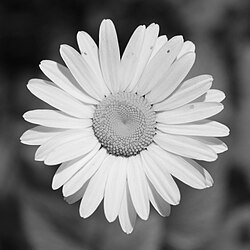
\includegraphics[width=\linewidth]{daisy_grises}
		\captionof{figure}{Original}
		\label{fig:ej1}
	\end{minipage}\hfill
	\begin{minipage}{0.3\linewidth}
		\centering
		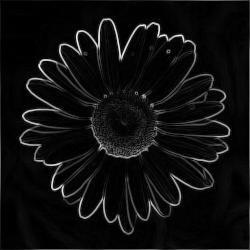
\includegraphics[width=\linewidth]{ej1a}
		\captionof{figure}{Prewitt}
		\label{fig:ej1a}
	\end{minipage}\hfill
	\begin{minipage}{0.3\linewidth}
		\centering
		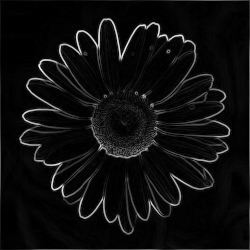
\includegraphics[width=\linewidth]{ej1b}
		\captionof{figure}{Sobel}
		\label{fig:ej1b}
	\end{minipage}
	
	\vfill
	\footnotesize \textcolor{lightgray}{(*) No se observan cambios signficatorios entre ambos operadores de gradiente.}
\end{frame}



\section{Ejercicio 2}

\begin{frame}
	\begin{center}
		\textcolor{unahurverde}{\textbf{Consigna 2:}}
	\end{center}
	\justifying
	Aplicar los detectores de borde del punto anterior a las mismas imágenes contaminadas con ruido.
\end{frame}

\begin{frame}[fragile]{Resultados con ruido}
	\justifying
	Al aplicar los \textcolor{unahurverde}{\textbf{Operadores de gradiente Prewitt y Sobel}} sobre la imagen con ruido Gaussiano ($40\%$ de contaminación y $\sigma=30$) de la Figura~\ref{fig:ej2}, se obtuvieron las versiones modificadas visibles en la Figura~\ref{fig:ej2a} y Figura~\ref{fig:ej2b}.
	\vspace{0.3cm}
	
	\centering
	\begin{minipage}{0.3\linewidth}
		\centering
		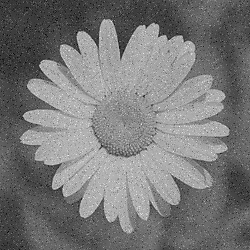
\includegraphics[width=\linewidth]{daisy_ruido}
		\captionof{figure}{Ruido}
		\label{fig:ej2}
	\end{minipage}\hfill
	\begin{minipage}{0.3\linewidth}
		\centering
		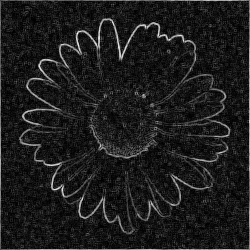
\includegraphics[width=\linewidth]{ej2a}
		\captionof{figure}{Prewitt}
		\label{fig:ej2a}
	\end{minipage}\hfill
	\begin{minipage}{0.3\linewidth}
		\centering
		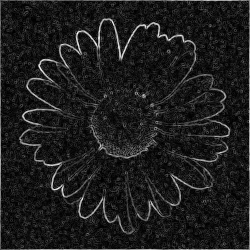
\includegraphics[width=\linewidth]{ej2b}
		\captionof{figure}{Sobel}
		\label{fig:ej2b}
	\end{minipage}
	
	\vfill
	\footnotesize \textcolor{lightgray}{(*) No se observan cambios signficatorios entre ambos operadores de gradiente.}
\end{frame}

\section{Ejercicio 3}

\begin{frame}
	\begin{center}
		\textcolor{unahurverde}{\textbf{Consigna 3:}}
	\end{center}
	\justifying
	Aplicar los detectores de borde del punto anterior a imágenes en color.
\end{frame}

\begin{frame}[fragile]{Resultados en imagen en color}
	\justifying
	Al aplicar los \textcolor{unahurverde}{\textbf{Operadores de gradiente Prewitt y Sobel}} sobre la imagen a color de la Figura~\ref{fig:ej3}, se obtuvieron las versiones modificadas visibles en la Figura~\ref{fig:ej3a} y Figura~\ref{fig:ej3b}.
	\vspace{0.3cm}
	
	\centering
	\begin{minipage}{0.3\linewidth}
		\centering
		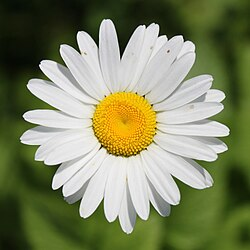
\includegraphics[width=\linewidth]{daisy}
		\captionof{figure}{Ruido}
		\label{fig:ej3}
	\end{minipage}\hfill
	\begin{minipage}{0.3\linewidth}
		\centering
		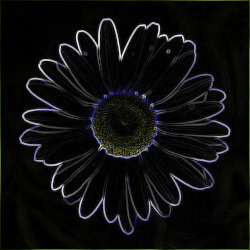
\includegraphics[width=\linewidth]{ej3a}
		\captionof{figure}{Prewitt}
		\label{fig:ej3a}
	\end{minipage}\hfill
	\begin{minipage}{0.3\linewidth}
		\centering
		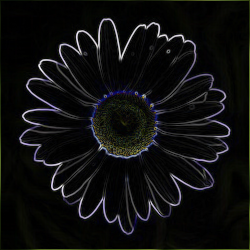
\includegraphics[width=\linewidth]{ej3b}
		\captionof{figure}{Sobel}
		\label{fig:ej3b}
	\end{minipage}
	
	\vfill
	\footnotesize \textcolor{lightgray}{(*) No se observan cambios signficatorios entre ambos operadores de gradiente.}
\end{frame}

\section{Ejercicio 4}

\begin{frame}
	\begin{center}
		\textcolor{unahurverde}{\textbf{Consigna 4:}}
	\end{center}
	\justifying
	Implementar los siguientes detectores de borde y aplicarlos a dos imágenes y a sus versiones contaminadas:
	\begin{enumerate}
		\item Método del Laplaciano.
		\item Método del Laplaciano agregándole evaluación de la pendiente.
		\item Método del Laplaciano del Gaussiano (Marr-Hildreth).
	\end{enumerate}
\end{frame}

\begin{frame}[fragile]{Operadores de segunda derivada}
	\justifying
	
	\begin{block}{Operador de Laplace}
		$f: \Re^2 \rightarrow \Re$
		\[
		\Delta f= \frac{\partial^2f}{\partial^2x} + \frac{\partial^2f}{\partial^2y}
		\]
	\end{block}
	
	\begin{block}{En imágenes se aproxima como:}
		\[
		\Delta I(x,y)= 4\ast I(x,y) - I(x-1,y) - I(x+1,y) - I(x,y-1) - I(x,y+1)
		\]
	\end{block}
	
	\vfill
	\footnotesize \textcolor{lightgray}{(*) El operador Laplaciano es la divergencia del gradiente.}
\end{frame}

\begin{frame}[fragile]{Máscara de Laplace y Cruces por cero}
	\justifying
	
	Como una máscara esto es:
	\begin{block}{Máscara de Laplace}
		\[
		\begin{bmatrix}
			0 & -1 & 0 \\
			-1 & 4 & -1 \\
			0 & -1 & 0
		\end{bmatrix}
		\]
	\end{block}
	
	Luego de convolucionar la imagen con la máscara de Laplace se deben encontrar los cruces por cero, el proceso es:
	
	\begin{itemize}
		\item Recorrer la imagen por filas y detectar los cambios de signos entre dos valores consecutivos, si hay un cambio asignar a ese pixel el valor 255, sino asignar el valor 0.
		\item Repetir para todas las filas.
	\end{itemize}
	
	Al encontrar los cruces por cero la imagen resulta en una binaria.
	
\end{frame}

\begin{frame}[fragile]{Código: Cruces por cero}
	\justifying

	\begin{lstlisting}[language=Python]
def encontrar_cruces_por_cero(imagen_np: np.ndarray) -> np.ndarray:
	m, n, _ = imagen_np.shape
	imagen_filtrada = np.zeros_like(imagen_np) # Predeterminadamente son cero y solo cambio los 255
	
	for i in range(m):
		for j in range(n - 1):
			for c in range(3):
				if imagen_np[i, j, c] * imagen_np[i, j + 1, c] < 0:
					imagen_filtrada[i, j] = 255
	
	return imagen_filtrada # Retorna una img binaria
	\end{lstlisting}
\end{frame}

\begin{frame}[fragile]{Evaluación de la pendiente}
	\justifying
	
	Al encontrar los cruces por cero se producen muchos puntos de borde falsos. Para corregir esto se mide el valor absoluto de la \textbf{pendiente del cruce} y si este valor supera cierto umbral se lo considera un borde.
	
	\begin{block}{Pendiente del cruce}
		\[
		|a + b|
		\]
	\end{block}
\end{frame}

\begin{frame}[fragile]{Código: Evaluación de pendiente}
	\justifying
	
	\begin{lstlisting}[language=Python]
def encontrar_cruces_por_cero_pendiente(imagen_np: np.ndarray, umbral=128) -> np.ndarray:
	m, n, _ = imagen_np.shape
	imagen_filtrada = np.zeros_like(imagen_np) # Predeterminadamente son cero y solo cambio los 255
	
	for i in range(m):
		for j in range(n - 1):
			for c in range(3):
				if abs(imagen_np[i, j, c]) + abs(imagen_np[i, j + 1, c]) > umbral:
					imagen_filtrada[i, j] = 255
	
	return imagen_filtrada # Retorna una img binaria
	\end{lstlisting}
\end{frame}

\begin{frame}[fragile]{Operador Laplaciano del Gaussiano}
	\justifying
	
	Para aplicar el Laplaciano del Gaussiano a una imagen debemos construir la máscara del LoG.
	
	\begin{block}{Calculo del Laplaciano del Gaussiano}
		\[
		\Delta G_\sigma(x, y) = \frac{1}{2\pi \sigma^3} e^{-\frac{x^2+y^2}{2\sigma^2}} (\frac{x^2+y^2}{\sigma^2} -2)
		\]
	\end{block}
	
	Luego se aplica la máscara a la imagen y se hacen los cruces por cero.
\end{frame}

\begin{frame}[fragile]{Resultados imagen 1}
	\justifying
	Sobre la imagen de la Figura~\ref{fig:ej4_img1} se aplicaron los siguientes detectores de borde:
	
	{\footnotesize
		\begin{itemize}
			\item Figura~\ref{fig:ej4a_img1}: Método del Laplaciano.
			\item Figura~\ref{fig:ej4b_img1}: Método del Laplaciano con evaluación de la pendiente con umbral=128.
			\item Figura~\ref{fig:ej4c_img1}: Método del Laplaciano del Gausiano (Marr-Hildreth) con $\sigma=1$.
		\end{itemize}
	}
	\vspace{0.3cm}
	
	\centering
	\begin{minipage}{0.24\linewidth}
		\centering
		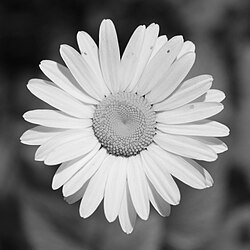
\includegraphics[width=\linewidth]{daisy_grises}
		\captionof{figure}{Original}
		\label{fig:ej4_img1}
	\end{minipage}\hfill
	\begin{minipage}{0.24\linewidth}
		\centering
		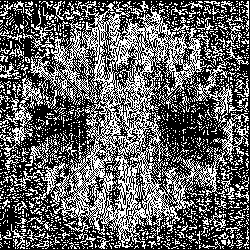
\includegraphics[width=\linewidth]{ej4a_img1}
		\captionof{figure}{Lap.}
		\label{fig:ej4a_img1}
	\end{minipage}\hfill
	\begin{minipage}{0.24\linewidth}
		\centering
		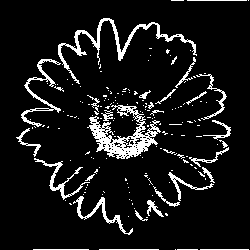
\includegraphics[width=\linewidth]{ej4b_img1}
		\captionof{figure}{Lap. P.}
		\label{fig:ej4b_img1}
	\end{minipage}\hfill
	\begin{minipage}{0.24\linewidth}
		\centering
		
\includegraphics[width=\linewidth]{ej4c_img1}
		\captionof{figure}{LoG}
		\label{fig:ej4c_img1}
	\end{minipage}

\end{frame}

\begin{frame}[fragile]{Resultados imagen 1 con ruido}
	\justifying
	Sobre la imagen de la Figura~\ref{fig:ej4_img1_gauss} la cual presenta ruido Gaussiano ($40\%$ de contaminación y $\sigma=30$), se aplicaron los siguientes detectores de borde:
	
	{\footnotesize
		\begin{itemize}
			\item Figura~\ref{fig:ej4a_img1_gauss}: Método del Laplaciano.
			\item Figura~\ref{fig:ej4b_img1_gauss}: Método del Laplaciano con evaluación de la pendiente con umbral=128.
			\item Figura~\ref{fig:ej4c_img1_gauss}: Método del Laplaciano del Gausiano (Marr-Hildreth) con $\sigma=1$.
		\end{itemize}
	}
	\vspace{0.3cm}
	
	\centering
	\begin{minipage}{0.24\linewidth}
		\centering
		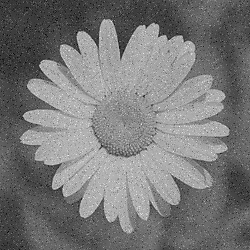
\includegraphics[width=\linewidth]{daisy_ruido}
		\captionof{figure}{Ruido}
		\label{fig:ej4_img1_gauss}
	\end{minipage}\hfill
	\begin{minipage}{0.24\linewidth}
		\centering
		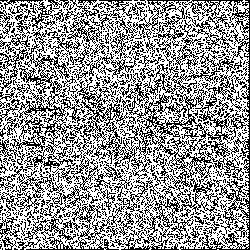
\includegraphics[width=\linewidth]{ej4a_img1_gauss}
		\captionof{figure}{Lap.}
		\label{fig:ej4a_img1_gauss}
	\end{minipage}\hfill
	\begin{minipage}{0.24\linewidth}
		\centering
		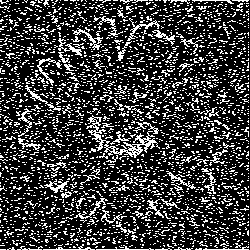
\includegraphics[width=\linewidth]{ej4b_img1_gauss}
		\captionof{figure}{Lap. P.}
		\label{fig:ej4b_img1_gauss}
	\end{minipage}\hfill
	\begin{minipage}{0.24\linewidth}
		\centering
		
\includegraphics[width=\linewidth]{ej4c_img1_gauss}
		\captionof{figure}{LoG}
		\label{fig:ej4c_img1_gauss}
	\end{minipage}
	
\end{frame}

\begin{frame}[fragile]{Resultados imagen 2}
	\justifying
	Sobre la imagen de la Figura~\ref{fig:ej4_img2} se aplicaron los siguientes detectores de borde:
	
	{\footnotesize
		\begin{itemize}
			\item Figura~\ref{fig:ej4a_img2}: Método del Laplaciano.
			\item Figura~\ref{fig:ej4b_img2}: Método del Laplaciano con evaluación de la pendiente con umbral=40.
			\item Figura~\ref{fig:ej4c_img2}: Método del Laplaciano del Gausiano (Marr-Hildreth) con $\sigma=1$.
		\end{itemize}
	}
	\vspace{0.3cm}
	
	\centering
	\begin{minipage}{0.24\linewidth}
		\centering
		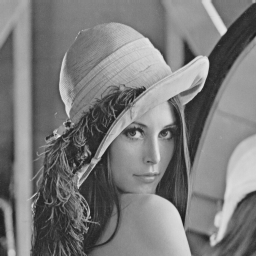
\includegraphics[width=\linewidth]{lena_grises}
		\captionof{figure}{Original}
		\label{fig:ej4_img2}
	\end{minipage}\hfill
	\begin{minipage}{0.24\linewidth}
		\centering
		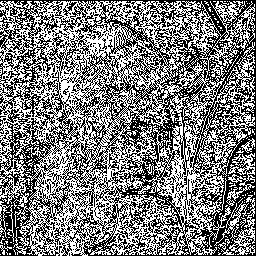
\includegraphics[width=\linewidth]{ej4a_img2}
		\captionof{figure}{Lap.}
		\label{fig:ej4a_img2}
	\end{minipage}\hfill
	\begin{minipage}{0.24\linewidth}
		\centering
		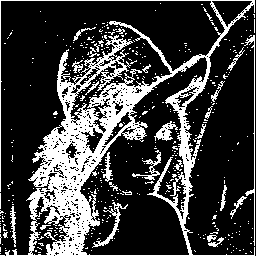
\includegraphics[width=\linewidth]{ej4b_img2}
		\captionof{figure}{Lap. P.}
		\label{fig:ej4b_img2}
	\end{minipage}\hfill
	\begin{minipage}{0.24\linewidth}
		\centering
		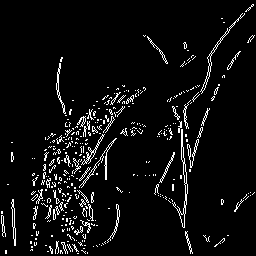
\includegraphics[width=\linewidth]{ej4c_img2}
		\captionof{figure}{LoG}
		\label{fig:ej4c_img2}
	\end{minipage}
	
\end{frame}

\begin{frame}[fragile]{Resultados imagen 2 con ruido}
	\justifying
	Sobre la imagen de la Figura~\ref{fig:ej4_img2_gauss} la cual presenta ruido Gaussiano ($40\%$ de contaminación y $\sigma=20$), se aplicaron los siguientes detectores de borde:
	
	{\footnotesize
		\begin{itemize}
			\item Figura~\ref{fig:ej4a_img2_gauss}: Método del Laplaciano.
			\item Figura~\ref{fig:ej4b_img2_gauss}: Método del Laplaciano con evaluación de la pendiente con umbral=40.
			\item Figura~\ref{fig:ej4c_img2_gauss}: Método del Laplaciano del Gausiano (Marr-Hildreth) con $\sigma=1$.
		\end{itemize}
	}
	\vspace{0.3cm}
	
	\centering
	\begin{minipage}{0.24\linewidth}
		\centering
		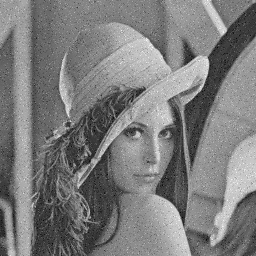
\includegraphics[width=\linewidth]{lena_gauss}
		\captionof{figure}{Ruido}
		\label{fig:ej4_img2_gauss}
	\end{minipage}\hfill
	\begin{minipage}{0.24\linewidth}
		\centering
		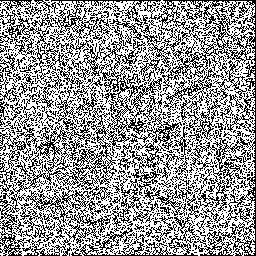
\includegraphics[width=\linewidth]{ej4a_img2_gauss}
		\captionof{figure}{Lap.}
		\label{fig:ej4a_img2_gauss}
	\end{minipage}\hfill
	\begin{minipage}{0.24\linewidth}
		\centering
		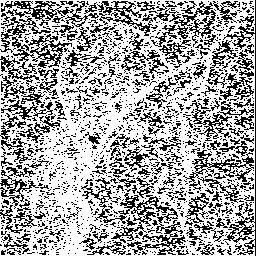
\includegraphics[width=\linewidth]{ej4b_img2_gauss}
		\captionof{figure}{Lap. P.}
		\label{fig:ej4b_img2_gauss}
	\end{minipage}\hfill
	\begin{minipage}{0.24\linewidth}
		\centering
		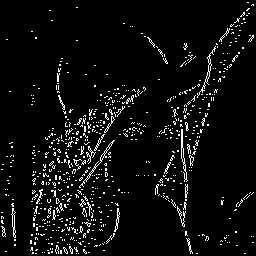
\includegraphics[width=\linewidth]{ej4c_img2_gauss}
		\captionof{figure}{LoG}
		\label{fig:ej4c_img2_gauss}
	\end{minipage}
	
\end{frame}

\section{Ejercicio 5}

\begin{frame}
	\begin{center}
		\textcolor{unahurverde}{\textbf{Consigna 5:}}
	\end{center}
	\justifying
	Implementar los métodos de Difusión Isotrópica y Anisotrópica. Aplicarlos a imágenes con ruido gaussiano y con ruido sal y pimienta. Comparar con el filtro de la mediana.
\end{frame}

\begin{frame}[fragile]{Difusión Isotrópica y Anisotrópica}
	\justifying
	
	La difusión isotrópica resuelve la ecuación del calor de conducción isotrópica:
	
	\begin{block}{Difusión Isotrópica}
		\[
		I_t(x,y,t) = \Delta I(x,y) = I_{xx} + I_{yy}
		\]
		Con la condición inicial: $I(x,y,0) = I_0$
	\end{block}
	
	Por otra parte la difusión anisotrópica
	
	\begin{block}{Difusión Anisotrópica}
		\[
		I_t(x,y,t) = \nabla \cdot (c(x,y,t) \nabla I(x,y))
		\]
		Con la condición inicial: $I(x,y,0) = I_0$
	\end{block}
	
	 c(x, y,t) es el coeficiente de conducción, el cual tiene como objetivo tener comportamiento distinto dependiendo si está en un borde o no (0 o 1 respectivamente).
	
	\vfill
	\footnotesize \textcolor{lightgray}{(*) Difusión del calor, con coeficiente constante o variable.}
\end{frame}

\begin{frame}[fragile]{Detectores de Borde}
	\justifying
	
	Para estimar la presencia de los bordes utilizaremos el modulo del gradiente:
	
	\begin{block}{Coeficiente}
		\[
		c(x,y,t) = g(|\nabla I|)
		\]
	\end{block}
	
	Y como detectores del mismo tenemos dos opciones:
	
	\begin{block}{Detector de Leclerc:}
		\[
		g(|\nabla I|) = e^{\frac{-|\nabla I|^2}{\sigma^2}}
		\]
	\end{block}
	
	\begin{block}{Detector de Lorentz:}
		\[
		g(|\nabla I|) = \frac{1}{\frac{-|\nabla I|^2}{\sigma^2}+1}
		\]
	\end{block}
	
	\vfill
	\footnotesize \textcolor{lightgray}{(*) .}
\end{frame}

\begin{frame}[fragile]{Implementación}
	\justifying
	
	La implementación consiste en calcular:
	
	\begin{block}{Implementación de Perona - Malik}
		\[
		I^{t+1}(x,y) = I^t(x,y) + \lambda (D_N c_N + D_E c_E + D_O c_O + D_S c_S)
		\]
		T veces.
	\end{block}
	
	\begin{block}{Donde}
		\[
		\begin{array}{cc}
			D_N = I(x, y+1) - I(x, y) & D_E = I(x-1, y) - I(x, y) \\[0.4em]
			D_O = I(x+1, y) - I(x, y) & D_S = I(x, y-1) - I(x, y)
		\end{array}
		\]
	\end{block}
	
	\begin{block}{Y los coeficientes se calculan como}
		\[
		c_N = g(D_N) \quad c_E = g(D_E) \quad c_O = g(D_O) \quad c_S = g(D_S)
		\]
		Si el filtro es isotrópico $c_N = c_E = c_O = c_S = 1$
	\end{block}

	\vfill
	\footnotesize \textcolor{lightgray}{(*) $\lambda = 0.25$}
\end{frame}

\begin{frame}[fragile]{Código: Detectores de borde}
	\justifying
	
	\begin{lstlisting}[language=Python]
def detector_de_leclerc(gradiente, sigma:int):
	return np.exp((-(gradiente**2))/sigma**2)

def detector_de_lorentz(gradiente, sigma:int):
	return 1/(((-(gradiente**2))/sigma**2) + 1)
	\end{lstlisting}
\end{frame}

\begin{frame}[fragile]{Código: Detectores de borde}
	\justifying
	Se ejecuta t veces el siguiente código para cada pixel (i, j, c) de la imagen:
	\begin{lstlisting}[language=Python]
# Gradientes
DN = img_filt[i, j + 1, c] - img_filt[i, j, c]
DE = img_filt[i - 1, j, c] - img_filt[i, j, c]
DO = img_filt[i + 1, j, c] - img_filt[i, j, c]
DS = img_filt[i, j - 1, c] - img_filt[i, j, c]

# Coeficientes
if isotropico: cN = cE = cO = cS = 1
else:
cN = detector_de_leclerc(DN, sigma)
cE = detector_de_leclerc(DE, sigma)
cO = detector_de_leclerc(DO, sigma)
cS = detector_de_leclerc(DS, sigma)

# Actualización
img_filt[i, j, c] += lamb * (DN * cN + DE * cE + DO * cO + DS * cS)
	\end{lstlisting}
\end{frame}

\begin{frame}[fragile]{Resultados Difusión con ruido Gauss}
	\justifying
	Sobre la imagen de la Figura~\ref{fig:ej5} la cual presenta ruido Gaussiano ($30\%$ de contaminación y $\sigma=20$), se aplicaron los siguientes métodos de eliminación de ruido:
	
	{\footnotesize
		\begin{itemize}
			\item Figura~\ref{fig:ej5a1}: Método de Difusión Isotrópica con $t=2$.
			\item Figura~\ref{fig:ej5b1}: Método de Difusión Anisotrópica con $t=5$ y $\sigma = 40$.
			\item Figura~\ref{fig:ej5c1}: Filtro de la Mediana con $k=3$.
		\end{itemize}
	}
	\vspace{0.3cm}
	
	\centering
	\begin{minipage}{0.24\linewidth}
		\centering
		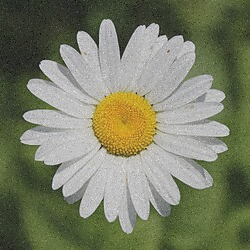
\includegraphics[width=\linewidth]{daisy_gauss}
		\captionof{figure}{Ruido}
		\label{fig:ej5}
	\end{minipage}\hfill
	\begin{minipage}{0.24\linewidth}
		\centering
		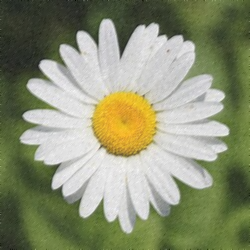
\includegraphics[width=\linewidth]{ej5a1}
		\captionof{figure}{Iso.}
		\label{fig:ej5a1}
	\end{minipage}\hfill
	\begin{minipage}{0.24\linewidth}
		\centering
		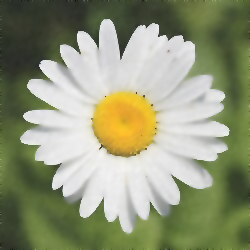
\includegraphics[width=\linewidth]{ej5b1}
		\captionof{figure}{Anis.}
		\label{fig:ej5b1}
	\end{minipage}\hfill
	\begin{minipage}{0.24\linewidth}
		\centering
		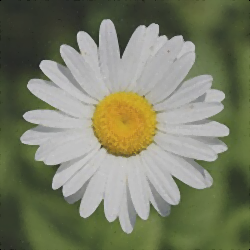
\includegraphics[width=\linewidth]{ej5c1}
		\captionof{figure}{Mediana}
		\label{fig:ej5c1}
	\end{minipage}
	
\end{frame}

\begin{frame}[fragile]{Resultados Difusión con ruido SyP}
	\justifying
	Sobre la imagen de la Figura~\ref{fig:ej5_syp} la cual presenta ruido Sal y Pimienta ($p=10$), se aplicaron los siguientes métodos de eliminación de ruido:
	
	{\footnotesize
		\begin{itemize}
			\item Figura~\ref{fig:ej5a2}: Método de Difusión Isotrópica con $t=15$.
			\item Figura~\ref{fig:ej5b2}: Método de Difusión Anisotrópica con $t=10$ y $\sigma = 50$.
			\item Figura~\ref{fig:ej5c2}: Filtro de la Mediana con $k=5$.
		\end{itemize}
	}
	\vspace{0.3cm}
	
	\centering
	\begin{minipage}{0.24\linewidth}
		\centering
		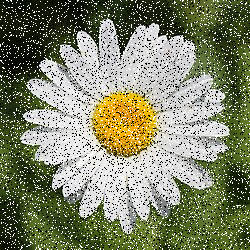
\includegraphics[width=\linewidth]{daisy_syp}
		\captionof{figure}{Ruido}
		\label{fig:ej5_syp}
	\end{minipage}\hfill
	\begin{minipage}{0.24\linewidth}
		\centering
		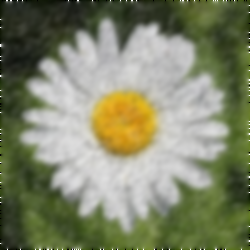
\includegraphics[width=\linewidth]{ej5a2}
		\captionof{figure}{Iso.}
		\label{fig:ej5a2}
	\end{minipage}\hfill
	\begin{minipage}{0.24\linewidth}
		\centering
		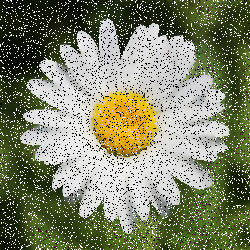
\includegraphics[width=\linewidth]{ej5b2}
		\captionof{figure}{Anis.}
		\label{fig:ej5b2}
	\end{minipage}\hfill
	\begin{minipage}{0.24\linewidth}
		\centering
		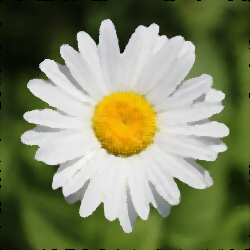
\includegraphics[width=\linewidth]{ej5c2}
		\captionof{figure}{Mediana}
		\label{fig:ej5c2}
	\end{minipage}
	
\end{frame}

\section{Ejercicio 6}

\begin{frame}
	\begin{center}
		\textcolor{unahurverde}{\textbf{Consigna 6:}}
	\end{center}
	\justifying
	Implementar el filtro bilateral. Aplicarlo a imágenes con ruido gaussiano y con ruido sal y pimienta. Comparar con el filtro de difusión anisotrópica.
\end{frame}

\begin{frame}[fragile]{Filtro Bilateral}
	\justifying
	
	Es un filtro donde el valor de cada pixel se reemplaza por el promedio pesado de los pixeles vecinos, el peso depende de la distancia de los pixeles al centro y de la diferencia en la intensidad del color.
	
	\begin{block}{Filtro Bilateral}
		\[
		I^{filt}(x) = \frac{1}{W_x} \sum_{x_i \in \Omega} I(x_i) G_{\sigma_s}(\|x_i - x\|) G_{\sigma_r}(\|I(x_i) - I(x)\|)
		\]
	\end{block}
	
	\begin{block}{Donde}
		\[
		W_x = \sum_{x_i \in \Omega} G_{\sigma_s}(\|x_i - x\|) G_{\sigma_r}(\|I(x_i) - I(x)\|)
		\]
		$W_x$ es un factor de normalización.
	\end{block}
	
\end{frame}

\begin{frame}[fragile]{Filtros $G_{\sigma_s}$ y $G_{\sigma_r}$}
	\justifying
	
	Luego los filtros se construyen como:
	
	\begin{block}{Filtros}
		\[
		 G_{\sigma_s} = e^{-\frac{(x^1-x^1_i)^2 + (x^2-x^2_i)^2}{2 \sigma_s^2}}
		\]
		\[
		G_{\sigma_r} = e^{-\frac{\|I(x) - I(x_i)\|^2}{2 \sigma_r^2}}
		\]
	\end{block}
	
	\vfill
	\footnotesize \textcolor{lightgray}{(*) Recordar que $I(x)$ es un vector.}
\end{frame}

\begin{frame}[fragile]{Código: Detectores de borde}
	\justifying
	Para cada pixel (i, j) se calcula su valor como:
	
	\begin{lstlisting}[language=Python]
region = imagen_padded[i:i+k, j:j+l, :]

dif = region - region[pad_h, pad_w, :]

Gr = np.exp(-(np.sum(dif**2, axis=2) / (2 * sigma_r**2)))

Wx = np.sum(Gs * Gr)

G = Gs * Gr
G = G[:, :, np.newaxis]

valor = (1 / Wx) * np.sum(region * G, axis=(0, 1))

imagen_filtrada[i, j, :] = valor
	\end{lstlisting}
	
	\vfill
	\footnotesize \textcolor{lightgray}{(*) Gs está calculado de ante mano por eficiencia.}
\end{frame}

\begin{frame}[fragile]{Resultados Bilateral con ruido Gaussiano}
	\justifying
	Sobre la imagen de la Figura~\ref{fig:ej6a} la cual presenta ruido Gaussiano ($30\%$ de contaminación y $\sigma=20$), se aplicaron los siguientes métodos de eliminación de ruido:
	
	{\footnotesize
		\begin{itemize}
			\item Figura~\ref{fig:ej6a1}: Filtro bilateral con $\sigma_s=10$ y $\sigma_r=50$.
			\item Figura~\ref{fig:ej6a2}: Método de Difusión Anisotrópica con $t=5$ y $\sigma = 40$.
		\end{itemize}
	}
	\vspace{0.3cm}
	
	\centering
	\begin{minipage}{0.3\linewidth}
		\centering
		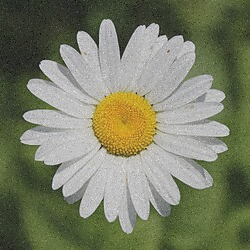
\includegraphics[width=\linewidth]{daisy_gauss}
		\captionof{figure}{Ruido}
		\label{fig:ej6a}
	\end{minipage}\hfill
	\begin{minipage}{0.3\linewidth}
		\centering
		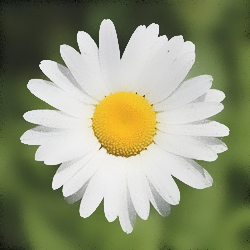
\includegraphics[width=\linewidth]{ej6a}
		\captionof{figure}{Bilateral}
		\label{fig:ej6a1}
	\end{minipage}\hfill
	\begin{minipage}{0.3\linewidth}
		\centering
		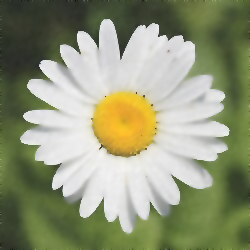
\includegraphics[width=\linewidth]{ej5b1}
		\captionof{figure}{Anis.}
		\label{fig:ej6a2}
	\end{minipage}
	
	Se observan cambios signficatorios entre ambos métodos, particularmente el Filtro Bilateral conserva mejor los bordes y la textura.
\end{frame}

\begin{frame}[fragile]{Resultados Bilateral con ruido Syp}
	\justifying
	Sobre la imagen de la Figura~\ref{fig:ej6b} la cual presenta ruido Sal y Pimienta ($p=10$), se aplicaron los siguientes métodos de eliminación de ruido:
	
	{\footnotesize
		\begin{itemize}
			\item Figura~\ref{fig:ej6b1}: Filtro bilateral con $\sigma_s=10$ y $\sigma_r=50$.
			\item Figura~\ref{fig:ej6b2}: Método de Difusión Anisotrópica con $t=10$ y $\sigma = 50$.
		\end{itemize}
	}
	\vspace{0.3cm}
	
	\centering
	\begin{minipage}{0.3\linewidth}
		\centering
		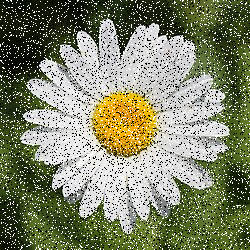
\includegraphics[width=\linewidth]{daisy_syp}
		\captionof{figure}{Ruido}
		\label{fig:ej6b}
	\end{minipage}\hfill
	\begin{minipage}{0.3\linewidth}
		\centering
		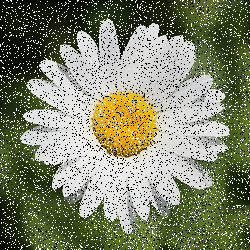
\includegraphics[width=\linewidth]{ej6b}
		\captionof{figure}{Bilateral}
		\label{fig:ej6b1}
	\end{minipage}\hfill
	\begin{minipage}{0.3\linewidth}
		\centering
		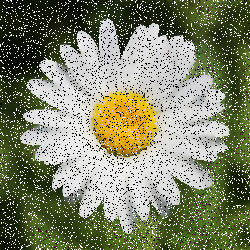
\includegraphics[width=\linewidth]{ej5b2}
		\captionof{figure}{Anis.}
		\label{fig:ej6b2}
	\end{minipage}
	
	Se observa que ninguno de estos métodos puede eliminar el ruido Sal y Pimienta.
\end{frame}

\section{Ejercicio 7}

\begin{frame}
	\begin{center}
		\textcolor{unahurverde}{\textbf{Consigna 7:}}
	\end{center}
	\justifying
	Implementar los siguientes algoritmos de umbralización y aplicarlos a dos imágenes y a sus versiones contaminadas:
	\begin{enumerate}
		\item Umbralización óptima iterativa.
		\item Método de umbralización de Otsu.
		\item Segmentación de imágenes en color (RGB) utilizando umbralización por bandas.
	\end{enumerate}
\end{frame}

\begin{frame}[fragile]{Código: Umbralización Iterativa}
	\justifying
	
	\begin{lstlisting}[language=Python]
for i in range(n):
	if T == T_anterior: break
	T_anterior = T
	
	imagen_binaria = aplicar_umbralizacion(imagen_np, T)
	nG1 = np.sum(imagen_binaria == 255)
	nG2 = np.sum(imagen_binaria == 0)
	
	m1 = (1 / nG1) * np.sum(imagen_np[imagen_binaria == 255])
	m2 = (1 / nG2) * np.sum(imagen_np[imagen_binaria == 0])
	
	T = int(0.5 * (m1 + m2))
	\end{lstlisting}
	
	\vfill
	\footnotesize \textcolor{lightgray}{(*) A manera de establecer un tope n=50.}
\end{frame}

\begin{frame}[fragile]{Código: Umbralización de Otsu}
	\justifying
	
	\begin{lstlisting}[language=Python]
intensidad = np.arange(256)
fi = np.bincount(datos_gris, minlength=256) 
N = datos_gris.size
pi = fi / N

P1 = np.zeros(256)
m = np.zeros(256)
for t in range(256):
	P1[t] = np.sum(pi[0:t+1])
	m[t] = np.sum(intensidad[0:t+1] * pi[0:t+1])
mG = m[255] # np.sum(intensidad * pi)

sigma_B = np.zeros(256)
for t in range(256):
	if P1[t] > 0 and P1[t] < 1:
		sigma_B[t] = ((mG * P1[t] - m[t])**2) / (P1[t] * (1 - P1[t]))
t_estrella = np.argmax(sigma_B)
resultado_np = aplicar_umbralizacion(imagen_np, t_estrella)
	\end{lstlisting}
\end{frame}

\begin{frame}[fragile]{Código: Umbralización por bandas}
	\justifying
	
	\begin{lstlisting}[language=Python]
def aplicar_umbralizacion_rgb(imagen_np: np.ndarray) -> np.ndarray:
	banda_r = imagen_np[:, :, 0]
	banda_g = imagen_np[:, :, 1]
	banda_b = imagen_np[:, :, 2]
	
	banda_r = aplicar_umbralizacion_de_otsu(banda_r)
	banda_g = aplicar_umbralizacion_de_otsu(banda_g)
	banda_b = aplicar_umbralizacion_de_otsu(banda_b)
	
	resultado_np = np.dstack([banda_r, banda_g, banda_b])
	
	# https://numpy.org/doc/stable/reference/generated/numpy.dstack.html
	return resultado_np
	\end{lstlisting}
\end{frame}

\begin{frame}[fragile]{Resultados Umbralización imagen 1}
	\justifying
	Sobre la imagen de la Figura~\ref{fig:ej7_img1} se aplicaron los siguientes métodos de umbralización:
	
	{\footnotesize
		\begin{itemize}
			\item Figura~\ref{fig:ej7a_img1}: Umbralización óptima iterativa, obteniendo $T=136$ en la iteración 3.
			\item Figura~\ref{fig:ej7b_img1}: Método umbralización de Otsu, obteniendo $T=136$.
			\item Figura~\ref{fig:ej7c_img1}: Segmentación de imágenes en color (RGB) utilizando umbralización por bandas, obteniendo estos umbrales para cada canal: R=136, G=142 y B=117.
		\end{itemize}
	}
	\vspace{0.3cm}
	
	\centering
	\begin{minipage}{0.24\linewidth}
		\centering
		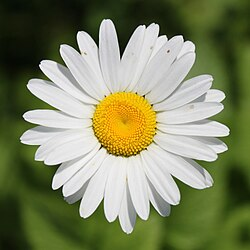
\includegraphics[width=\linewidth]{daisy}
		\captionof{figure}{Original}
		\label{fig:ej7_img1}
	\end{minipage}\hfill
	\begin{minipage}{0.24\linewidth}
		\centering
		
\includegraphics[width=\linewidth]{ej7a_img1}
		\captionof{figure}{Iter.}
		\label{fig:ej7a_img1}
	\end{minipage}\hfill
	\begin{minipage}{0.24\linewidth}
		\centering
		
\includegraphics[width=\linewidth]{ej7b_img1}
		\captionof{figure}{Otsu.}
		\label{fig:ej7b_img1}
	\end{minipage}\hfill
	\begin{minipage}{0.24\linewidth}
		\centering
		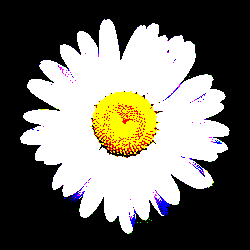
\includegraphics[width=\linewidth]{ej7c_img1}
		\captionof{figure}{Seg.}
		\label{fig:ej7c_img1}
	\end{minipage}
	
\end{frame}

\begin{frame}[fragile]{Resultados Umbralización imagen 1 con ruido}
	\justifying
	Sobre la imagen de la Figura~\ref{fig:ej7_img1_gauss} contaminada, se aplicaron los siguientes métodos de umbralización:
	
	{\footnotesize
		\begin{itemize}
			\item Figura~\ref{fig:ej7a_img1_gauss}: Umbralización óptima iterativa, obteniendo $T=128$ en la iteración 3.
			\item Figura~\ref{fig:ej7b_img1_gauss}: Método umbralización de Otsu, obteniendo $T=128$.
			\item Figura~\ref{fig:ej7c_img1_gauss}: Segmentación de imágenes en color (RGB) utilizando umbralización por bandas, obteniendo estos umbrales para cada canal: R=128, G=132 y B=116.
		\end{itemize}
	}
	\vspace{0.3cm}
	
	\centering
	\begin{minipage}{0.24\linewidth}
		\centering
		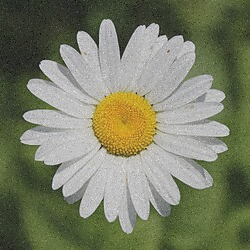
\includegraphics[width=\linewidth]{daisy_gauss}
		\captionof{figure}{Ruido}
		\label{fig:ej7_img1_gauss}
	\end{minipage}\hfill
	\begin{minipage}{0.24\linewidth}
		\centering
		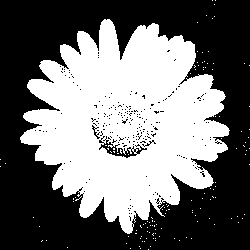
\includegraphics[width=\linewidth]{ej7a_img1_gauss}
		\captionof{figure}{Iter.}
		\label{fig:ej7a_img1_gauss}
	\end{minipage}\hfill
	\begin{minipage}{0.24\linewidth}
		\centering
		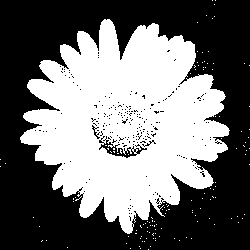
\includegraphics[width=\linewidth]{ej7b_img1_gauss}
		\captionof{figure}{Otsu.}
		\label{fig:ej7b_img1_gauss}
	\end{minipage}\hfill
	\begin{minipage}{0.24\linewidth}
		\centering
		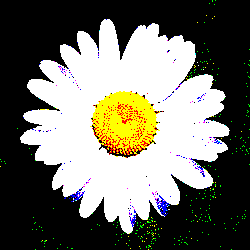
\includegraphics[width=\linewidth]{ej7c_img1_gauss}
		\captionof{figure}{Seg.}
		\label{fig:ej7c_img1_gauss}
	\end{minipage}
	
\end{frame}

\begin{frame}[fragile]{Resultados Umbralización imagen 2}
	\justifying
	Sobre la imagen de la Figura~\ref{fig:ej7_img2} se aplicaron los siguientes métodos de umbralización:
	
	{\footnotesize
		\begin{itemize}
			\item Figura~\ref{fig:ej7a_img2}: Umbralización óptima iterativa, obteniendo $T=123$ en la iteración 4.
			\item Figura~\ref{fig:ej7b_img2}: Método umbralización de Otsu, obteniendo $T=125$.
			\item Figura~\ref{fig:ej7c_img2}: Segmentación de imágenes en color (RGB) utilizando umbralización por bandas, obteniendo estos umbrales para cada canal: R=119, G=126 y B=138.
		\end{itemize}
	}
	\vspace{0.3cm}
	
	\centering
	\begin{minipage}{0.24\linewidth}
		\centering
		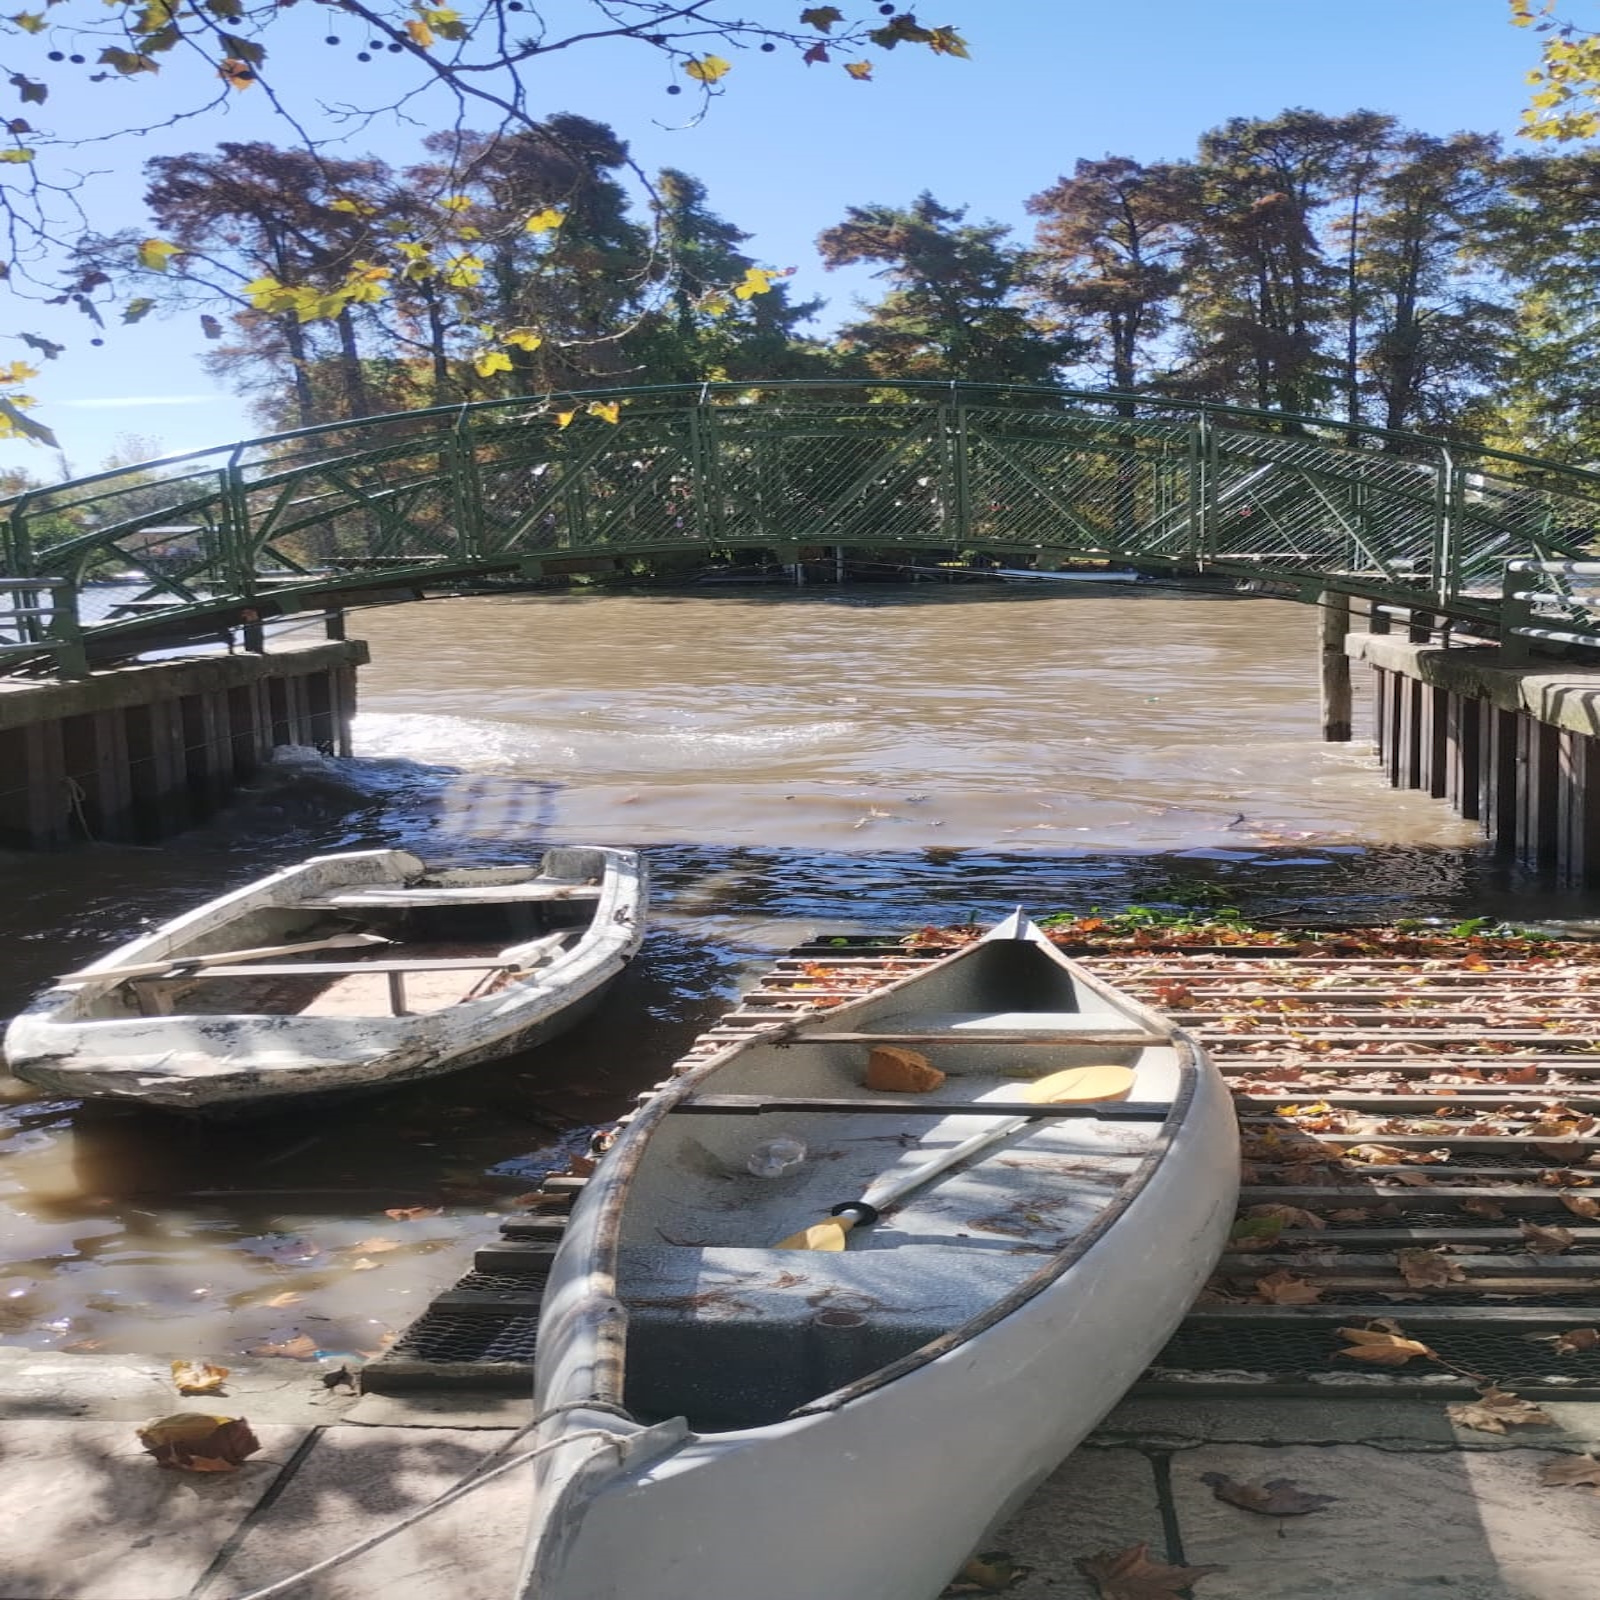
\includegraphics[width=\linewidth]{tigre}
		\captionof{figure}{Original}
		\label{fig:ej7_img2}
	\end{minipage}\hfill
	\begin{minipage}{0.24\linewidth}
		\centering
		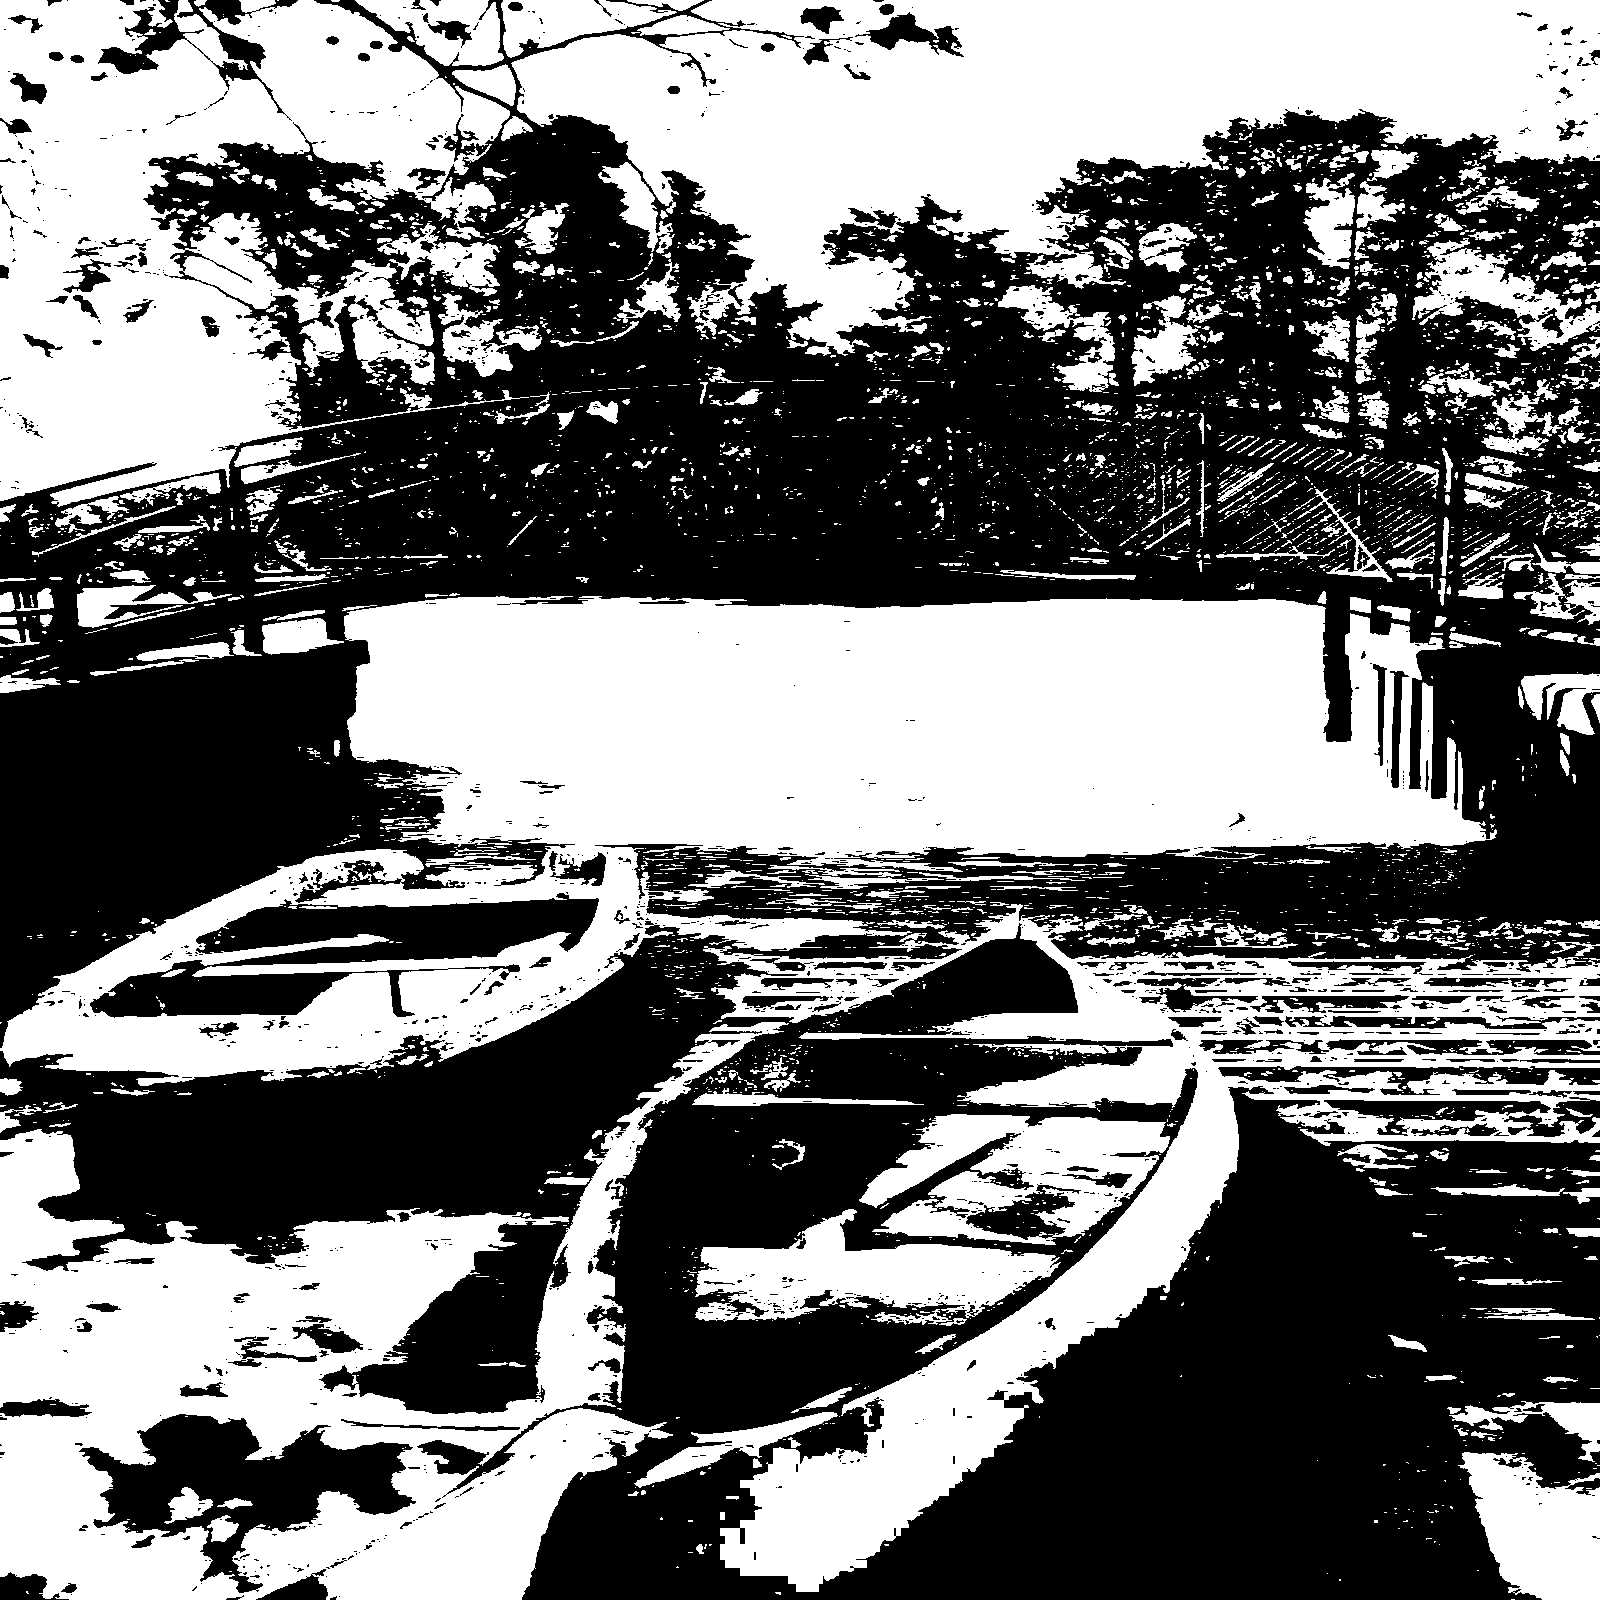
\includegraphics[width=\linewidth]{ej7a_img2}
		\captionof{figure}{Iter.}
		\label{fig:ej7a_img2}
	\end{minipage}\hfill
	\begin{minipage}{0.24\linewidth}
		\centering
		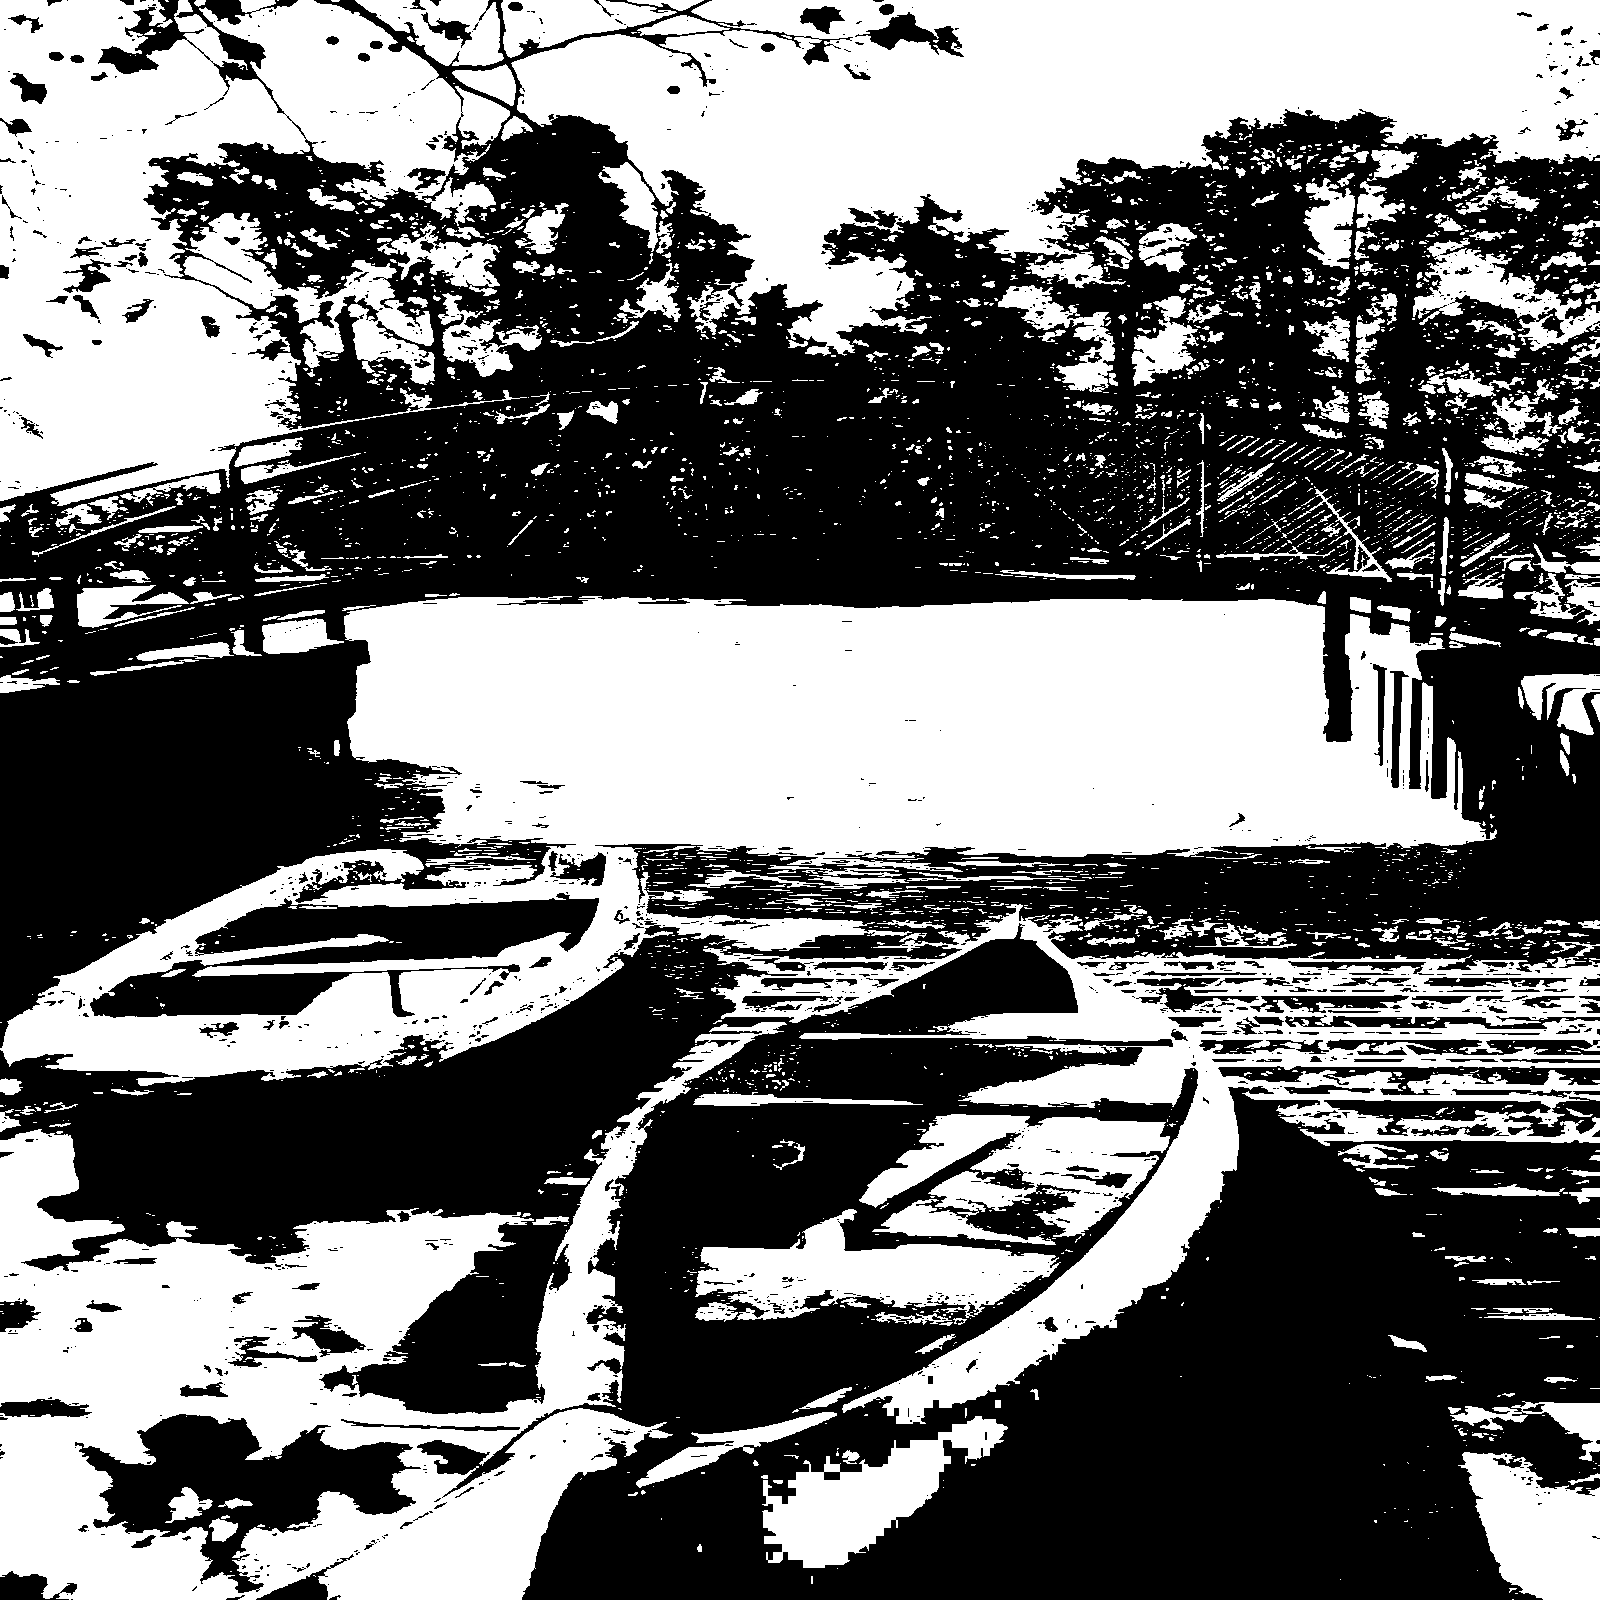
\includegraphics[width=\linewidth]{ej7b_img2}
		\captionof{figure}{Otsu.}
		\label{fig:ej7b_img2}
	\end{minipage}\hfill
	\begin{minipage}{0.24\linewidth}
		\centering
		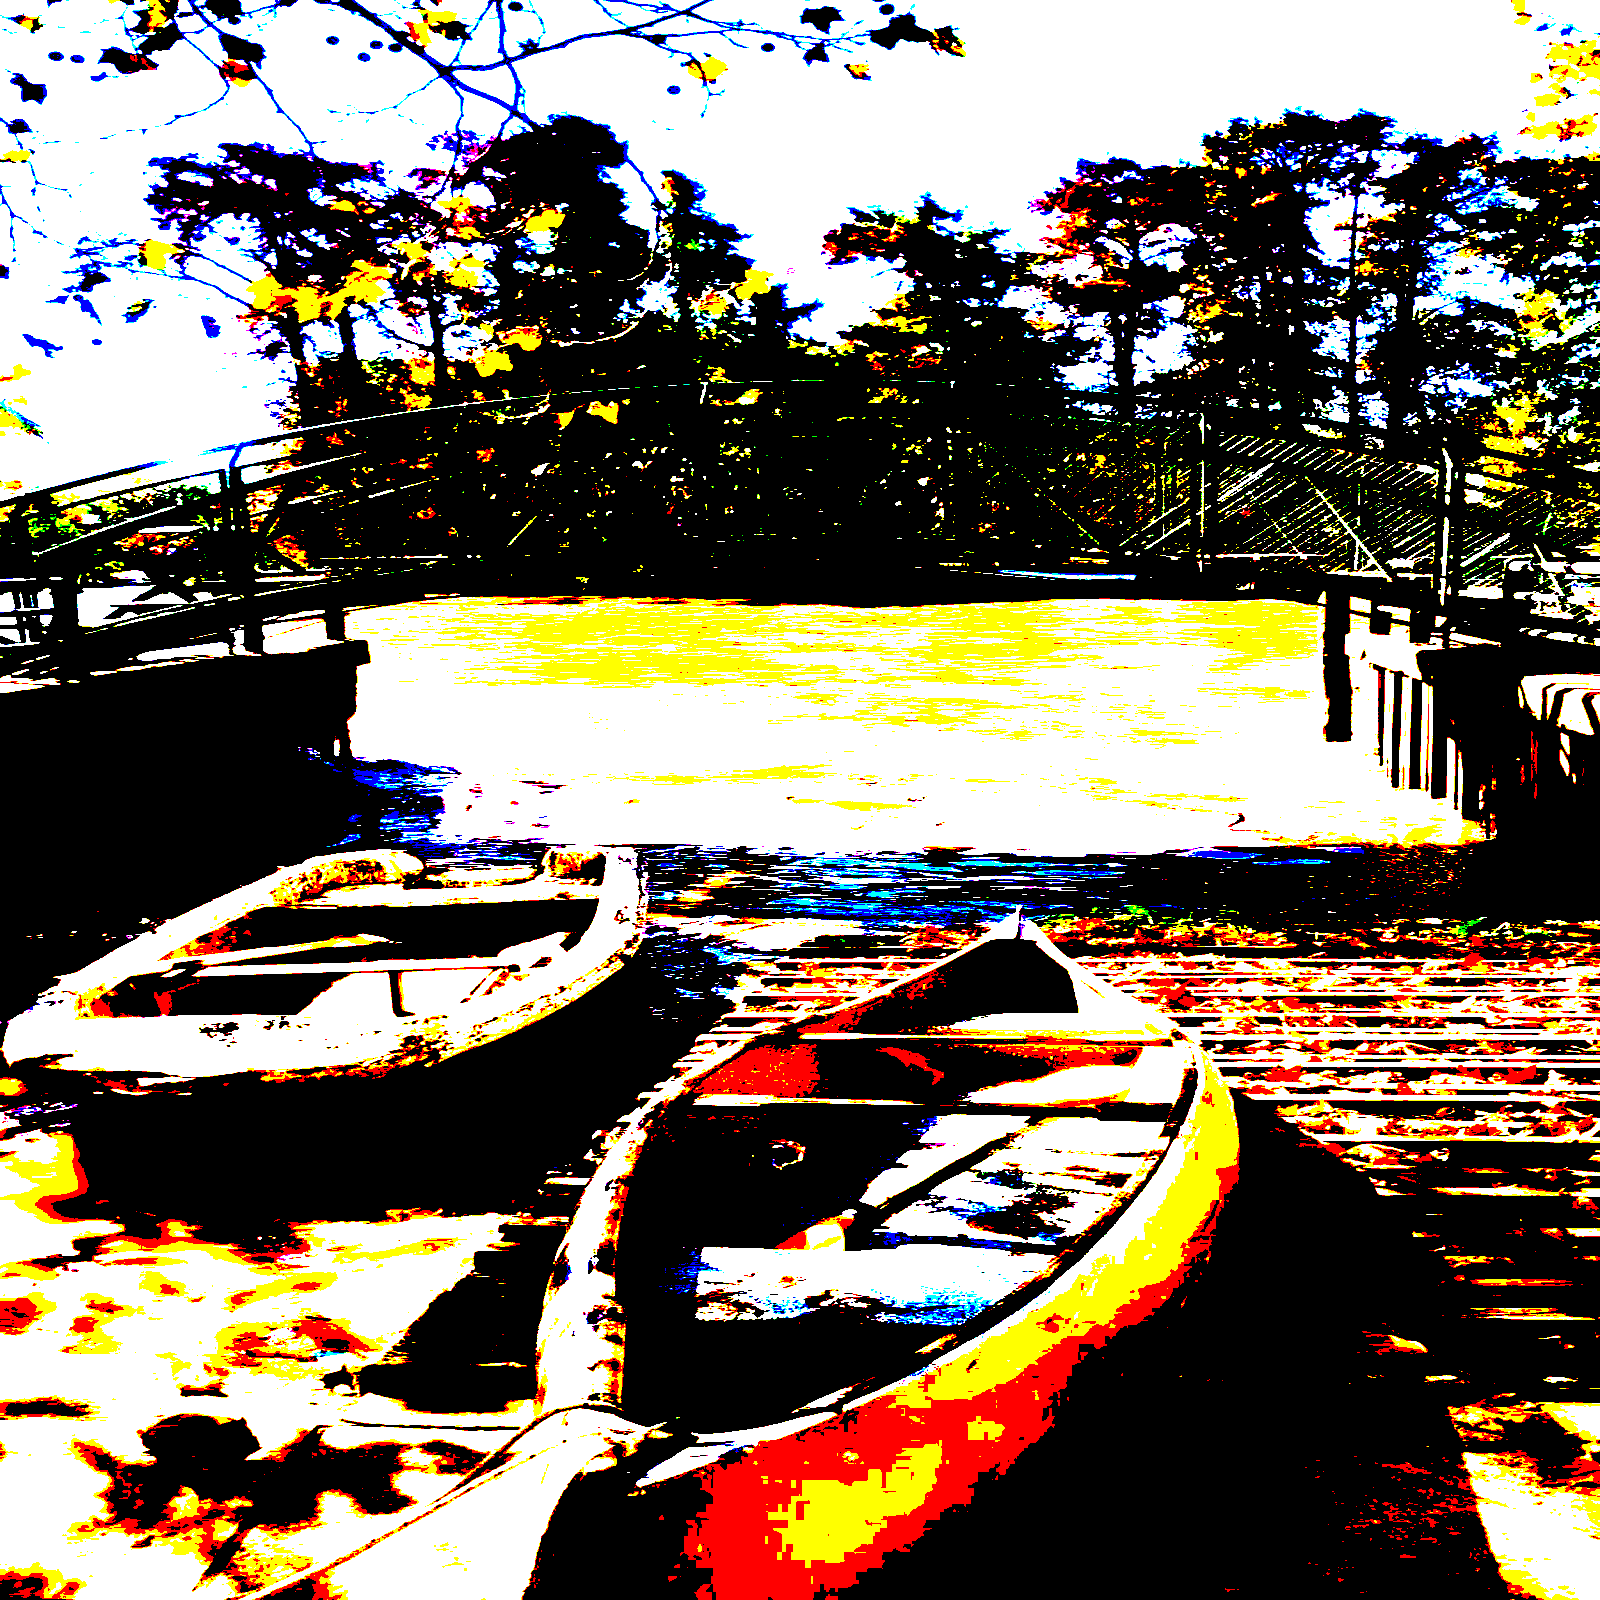
\includegraphics[width=\linewidth]{ej7c_img2}
		\captionof{figure}{Seg.}
		\label{fig:ej7c_img2}
	\end{minipage}
	
\end{frame}

\begin{frame}[fragile]{Resultados Umbralización imagen 2 con ruido}
	\justifying
	Sobre la imagen de la Figura~\ref{fig:ej7_img2_gauss} se aplicaron los siguientes métodos de umbralización:
	
	{\footnotesize
		\begin{itemize}
			\item Figura~\ref{fig:ej7a_img2_gauss}: Umbralización óptima iterativa, obteniendo $T=113$ en la iteración 2.
			\item Figura~\ref{fig:ej7b_img2_gauss}: Método umbralización de Otsu, obteniendo $T=115$.
			\item Figura~\ref{fig:ej7c_img2_gauss}: Segmentación de imágenes en color (RGB) utilizando umbralización por bandas, obteniendo estos umbrales para cada canal: R=112, G=115 y B=122.
		\end{itemize}
	}
	\vspace{0.3cm}
	
	\centering
	\begin{minipage}{0.24\linewidth}
		\centering
		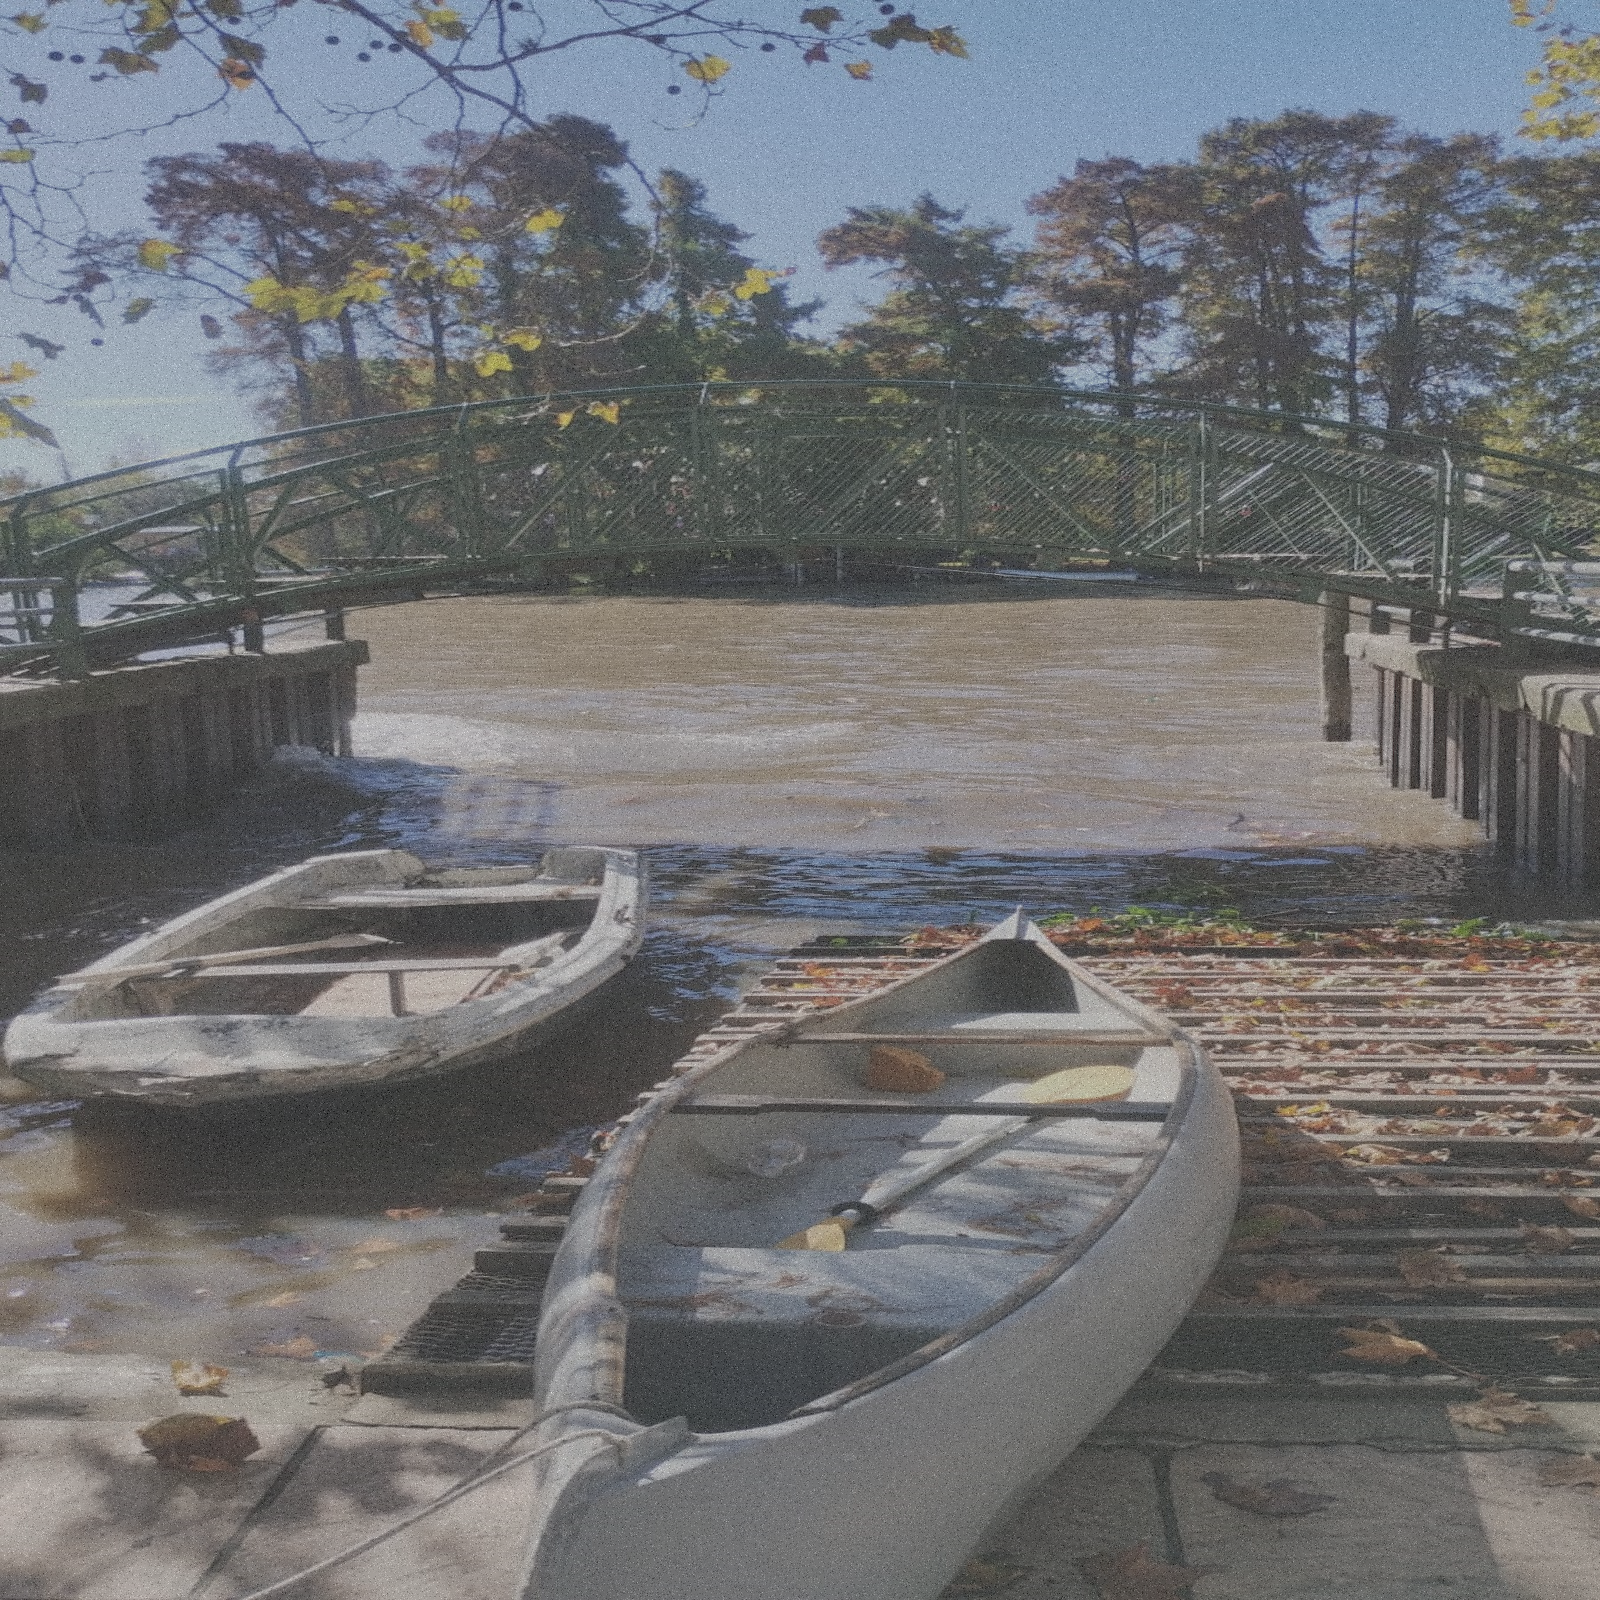
\includegraphics[width=\linewidth]{tigre_gauss}
		\captionof{figure}{Ruido}
		\label{fig:ej7_img2_gauss}
	\end{minipage}\hfill
	\begin{minipage}{0.24\linewidth}
		\centering
		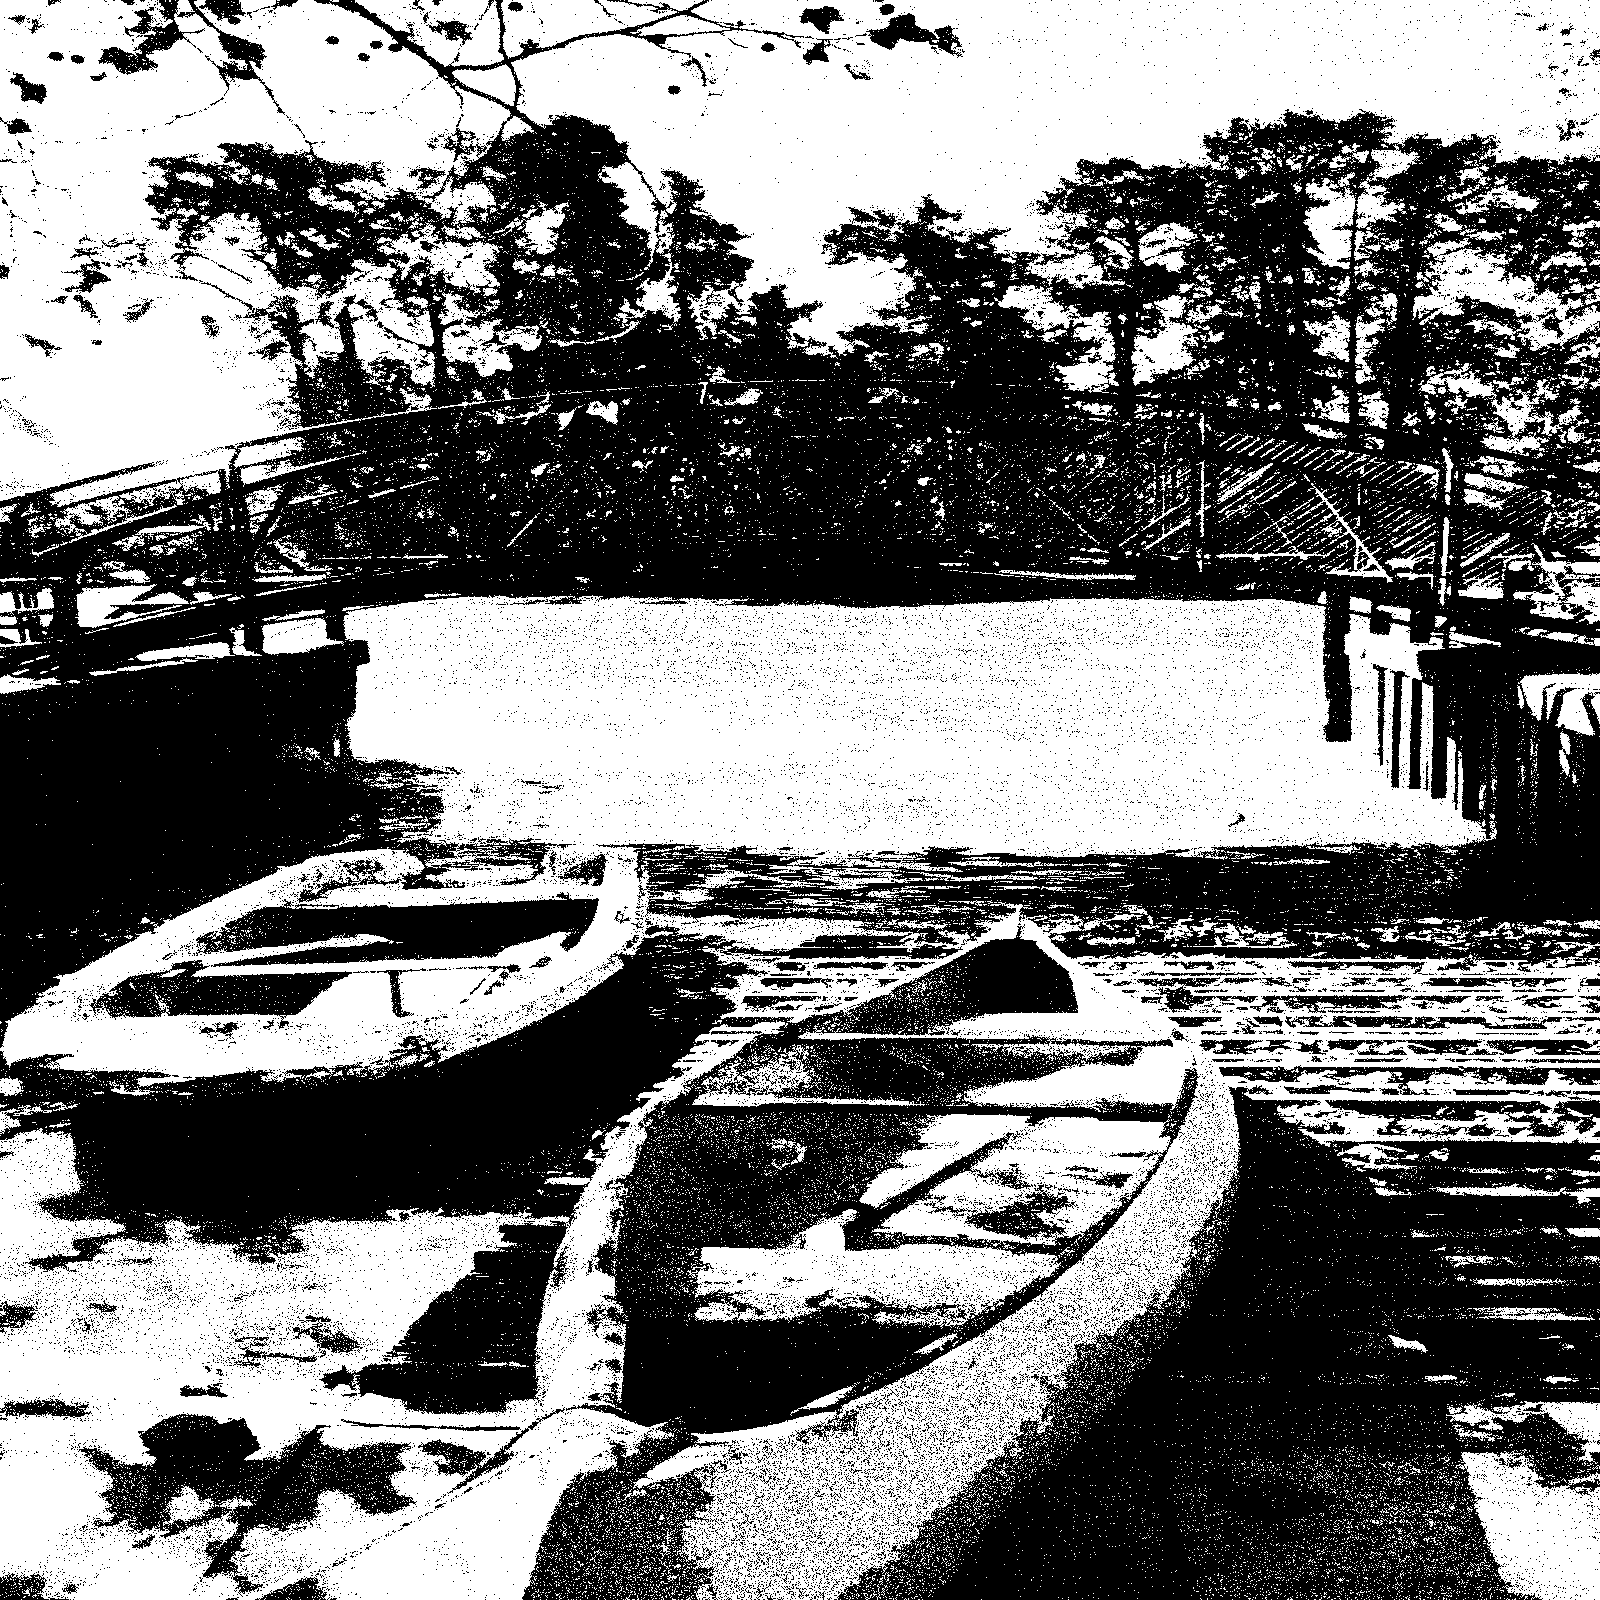
\includegraphics[width=\linewidth]{ej7a_img2_gauss}
		\captionof{figure}{Iter.}
		\label{fig:ej7a_img2_gauss}
	\end{minipage}\hfill
	\begin{minipage}{0.24\linewidth}
		\centering
		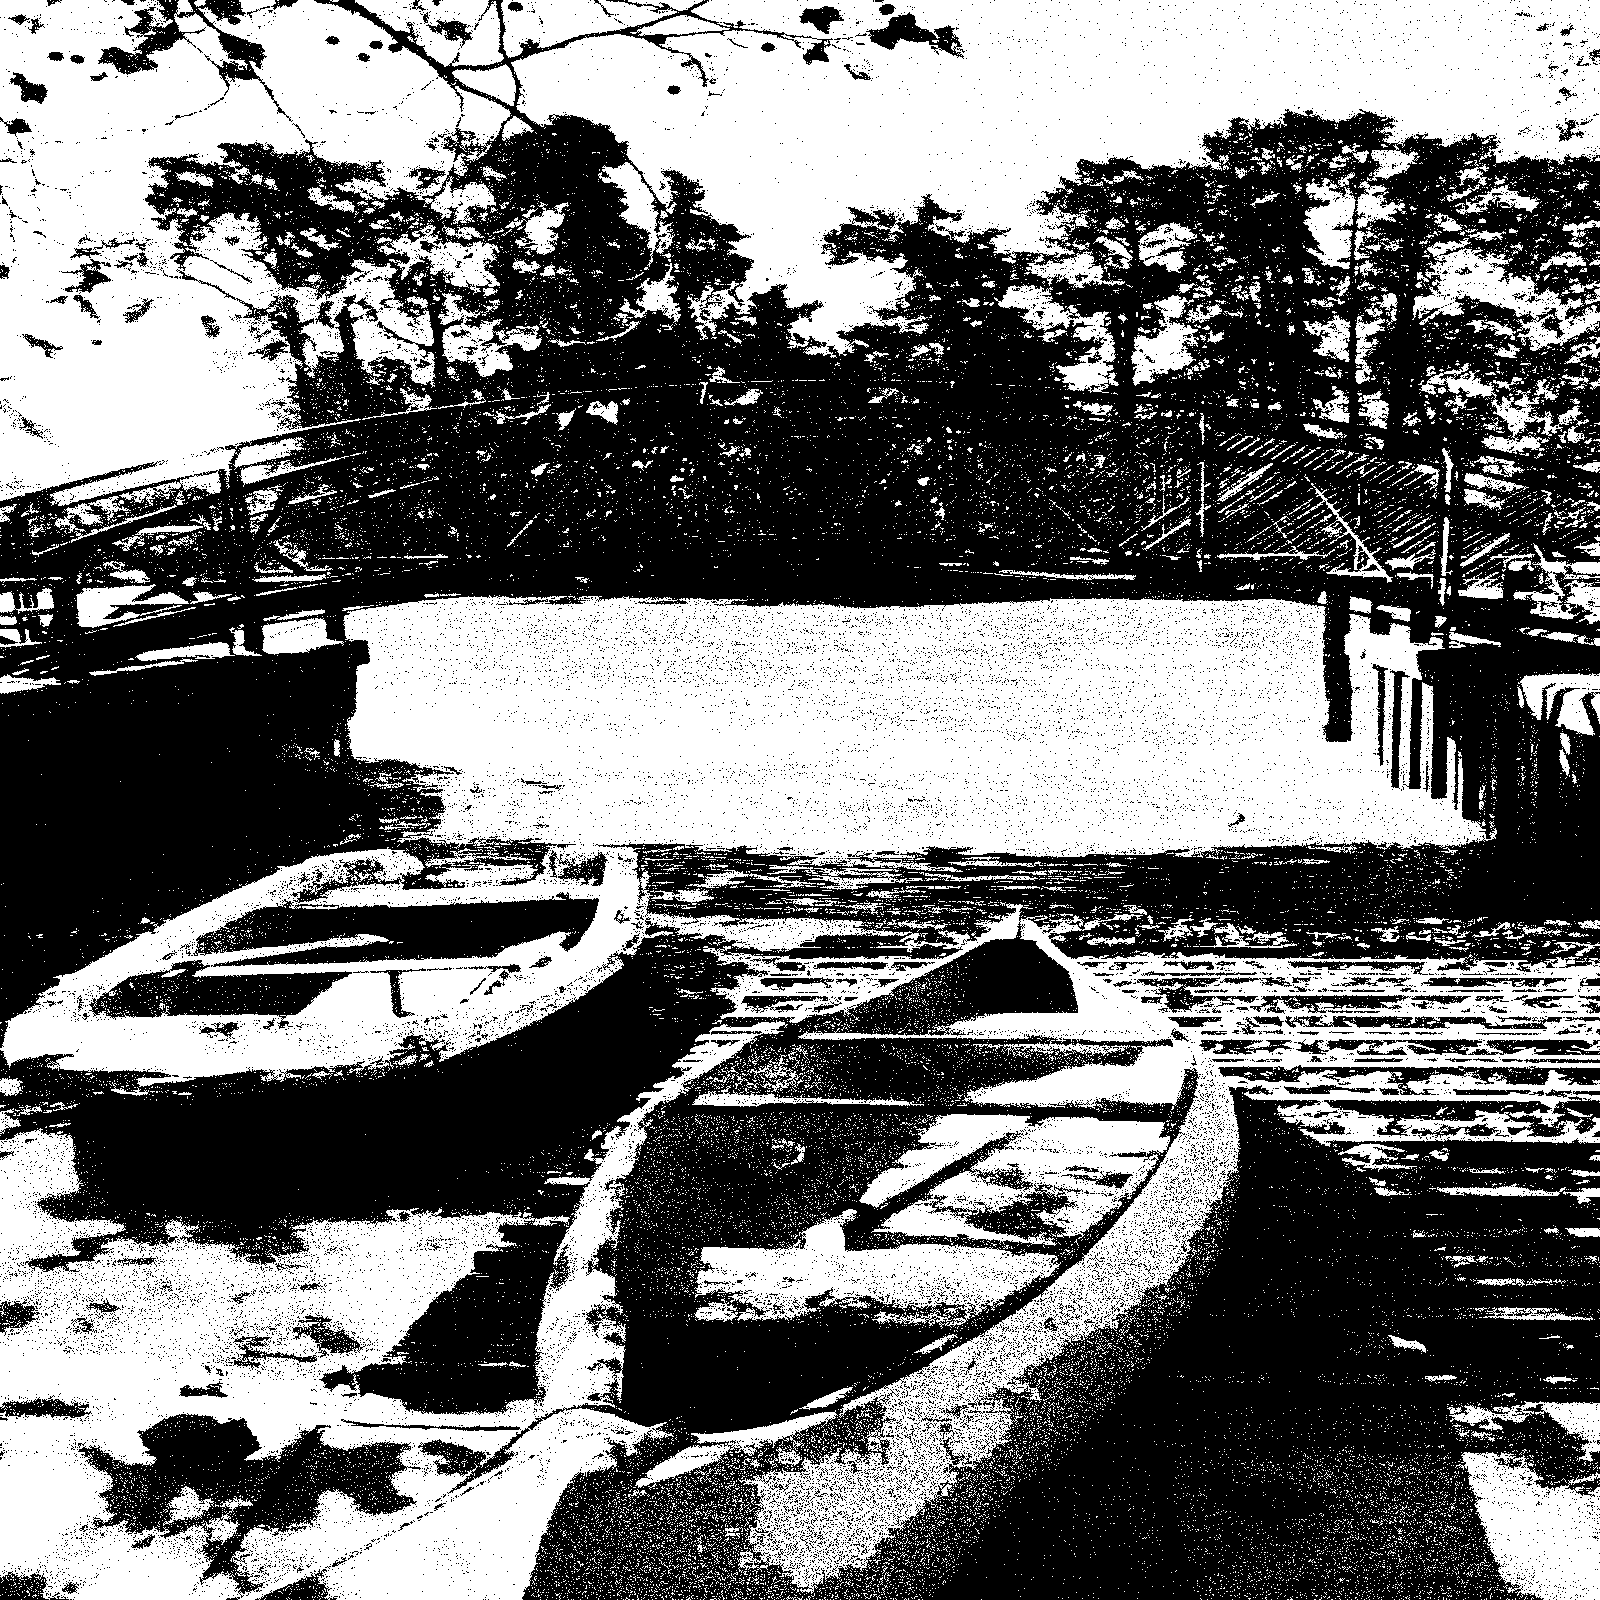
\includegraphics[width=\linewidth]{ej7b_img2_gauss}
		\captionof{figure}{Otsu.}
		\label{fig:ej7b_img2_gauss}
	\end{minipage}\hfill
	\begin{minipage}{0.24\linewidth}
		\centering
		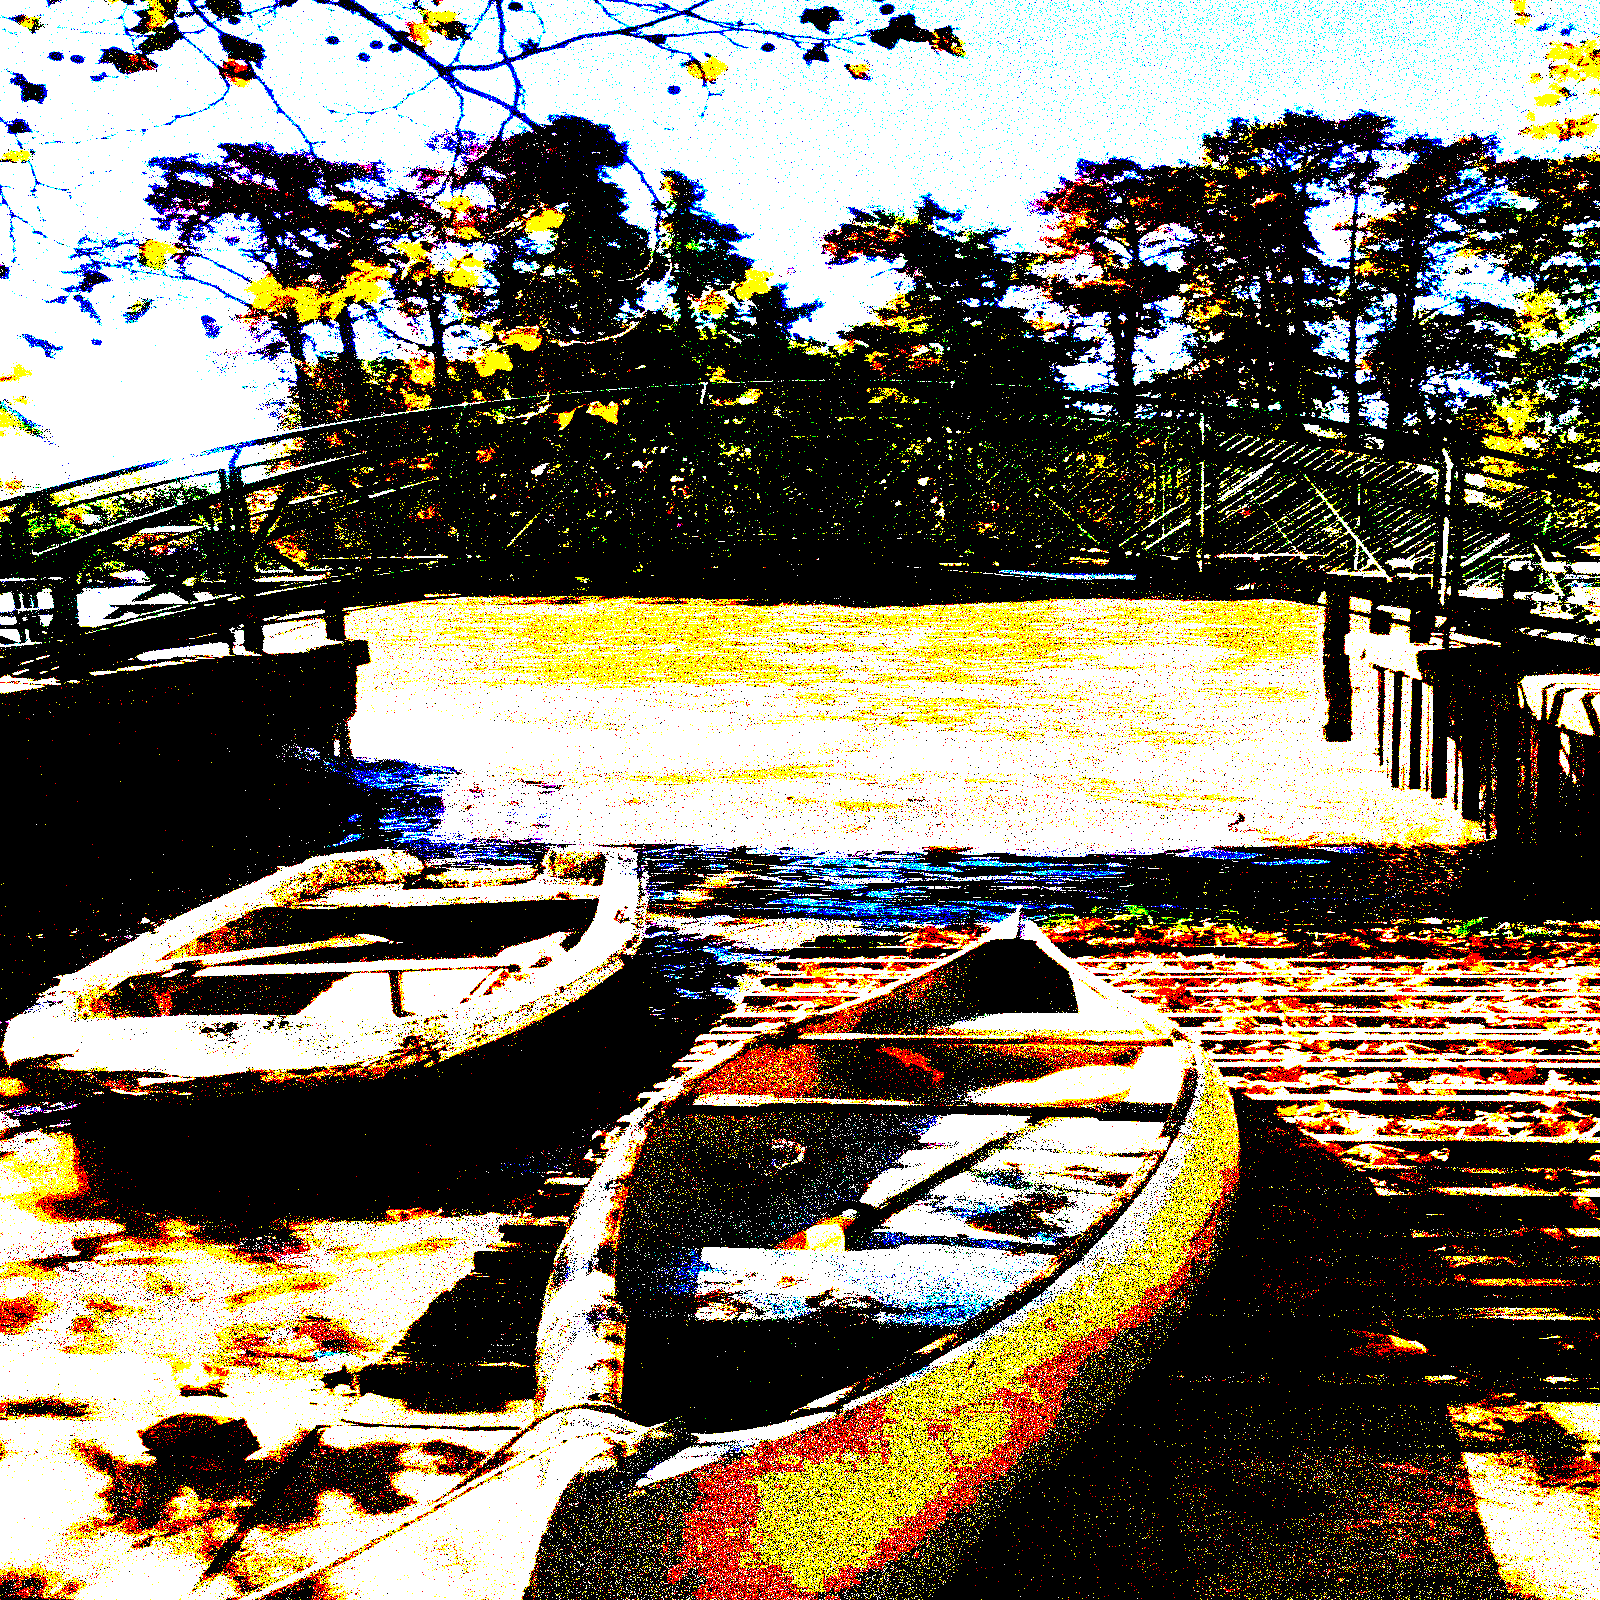
\includegraphics[width=\linewidth]{ej7c_img2_gauss}
		\captionof{figure}{Seg.}
		\label{fig:ej7c_img2_gauss}
	\end{minipage}
	
\end{frame}

\section{Repositorio}

\begin{frame}{Repositorio de GitHub}
	\justifying
	Todo el código y los resultados de este trabajo están disponibles en mi repositorio de GitHub: 
	
	\vspace{0.5cm}
	\centering
	\href{https://github.com/matias-cisnero/procesamiento_imagenes}{\textcolor{unahurverde}{\textbf{https://github.com/matias-cisnero/procesamiento\_imagenes}}}
\end{frame}

\section{Bibliografía}
	
\begin{frame}{Referencias}
	\tiny
	\begin{thebibliography}{10}
		\beamertemplateonlinebibitems
		\bibitem{numpy-broadcasting}
		NumPy Documentation: Broadcasting. 
		\newblock \url{https://numpy.org/doc/stable/user/basics.broadcasting.html}
		
		\bibitem{wikimedia-leucanthemum}
		Imagen \textit{“Leucanthemum vulgare Blüte”} por Mariofan13. 
		\newblock Wikimedia Commons. Licencia \textit{CC BY-SA 3.0 Unported}. 
		\newblock \href{https://commons.wikimedia.org/wiki/File:Leucanthemum_vulgare_Bl\%C3\%BCte.JPG}{Ver imagen en Wikimedia Commons}
		
		\beamertemplatebookbibitems
		\bibitem{digital-image-processing}
		Gonzalez, R. and Woods, R. (2018). Digital Image Processing. Pearson Education 4th Edition, New York.
	\end{thebibliography}
\end{frame}

\begin{frame}{}
	\centering
	{\huge ¡Gracias!}\\
	\vspace{1cm}
	
\includegraphics[width=0.2\textwidth]{UNAHUR.png}
\end{frame}
	
\end{document}
